\documentclass[a4paper]{article}
\usepackage[T1]{fontenc}			% pacchetto per \chapter
\usepackage[italian]{babel}
\usepackage[italian]{isodate}  		% formato delle date in italiano
\usepackage{graphicx}				% gestione delle immagini
\usepackage{amsfonts}
\usepackage{booktabs}				% tabelle di qualità superiore
\usepackage{amsmath}				% pacchetto matematica
\usepackage{mathtools}				% per sottolineare sotto le equazioni
\usepackage{stmaryrd} 				% per '\llbracket' e '\rrbracket'
\usepackage{amsthm}					% teoremi migliorati
\usepackage{enumitem}				% gestione delle liste
\usepackage{pifont}					% pacchetto con elenchi carini
\usepackage{enumitem}				% pacchetto per elenchi con lettere dell'alfabeto
\usepackage{cancel}					% per cancellare delle espressioni matematiche
\usepackage{caption}
\usepackage[]{mdframed}


% draw a frame around given text
\newcommand{\framedtext}[1]{%
\par%
\noindent\fbox{%
    \parbox{\dimexpr\linewidth-2\fboxsep-2\fboxrule}{#1}%
}%
}



\usepackage[x11names]{xcolor}		% pacchetto colori RGB
% Link ipertestuali per l'indice
\usepackage{xcolor}
\usepackage[linkcolor=black, citecolor=blue, urlcolor=cyan]{hyperref}
\hypersetup{
	colorlinks=true
}

\usepackage{tikz}
\newcommand{\MyTikzmark}[2]{%
	\tikz[overlay,remember picture,baseline] \node [anchor=base] (#1) {#2};%
}
\newcommand{\DrawVLine}[3][]{%
	\begin{tikzpicture}[overlay,remember picture]
		\draw[shorten <=0.3ex, #1] (#2.north) -- (#3.south);
	\end{tikzpicture}
}
\newcommand{\DrawHLine}[3][]{%
	\begin{tikzpicture}[overlay,remember picture]
		\draw[shorten <=0.2em, #1] (#2.west) -- (#3.east);
	\end{tikzpicture}
}


%\usepackage{showframe}				% visualizzazione bordi
%\usepackage{showkeys}				% visualizzazione etichetta

\newtheorem{theorem}{\textcolor{Red3}{\underline{Teorema}}}
\newtheorem{lemma}{Lemma}
\renewcommand{\qedsymbol}{QED}
\newcommand{\exec}[1]{\llbracket #1\:\rrbracket}
\newcommand{\dquotes}[1]{``#1''}
\newcommand{\longline}{\noindent\rule{\textwidth}{0.4pt}}
\newcommand{\circledtext}[1]{\raisebox{.5pt}{\textcircled{\raisebox{-.9pt}{#1}}}}

\newenvironment{rowequmat}[1]{\left(\array{@{}#1@{}}}{\endarray\right)}
\newenvironment{rowequmatbra}[1]{\left[\array{@{}#1@{}}}{\endarray\right]}

\begin{document}
	\author{VR443470}
	\title{Guida agli Esami di Analisi II}
	\date{\printdayoff\today}
	\maketitle

	\newpage

	% indice
	\tableofcontents

	\newpage

	\section{Esercizio 1 - Problema di Cauchy}

	\subsection{Problema di Cauchy - Soluzione}

	Il primo esercizio è sempre uguale e riguarda il problema di Cauchy. Un esempio di testo tratto dal tema d'esame del 25/06/2021: \textcolor{Green4}{\textbf{\emph{Si trovi una soluzione locale del seguente problema di Cauchy e si determini l'intervallo massimale in cui tale soluzione è definita.}}}
	\begin{equation*}
		\begin{cases}
			y' + \dfrac{y^{3}}{x^{2} + 1} = 0 \\
			\\
			y\left(0\right) = 1
		\end{cases}
	\end{equation*}
	Il \textbf{primo passo} è esplicitare la derivata, per cui:
	\begin{equation*}
		\begin{cases}
			y' + \dfrac{y^{3}}{x^{2} + 1} = 0 \\
			\\
			y\left(0\right) = 1
		\end{cases}
		\longrightarrow
		\begin{cases}
			y' = -\dfrac{y^{3}}{x^{2} + 1} \\
			\\
			y\left(0\right) = 1
		\end{cases}
	\end{equation*}
	Il \textbf{secondo passo} è risolvere l'integrale per ciascuna parte:
	\begin{equation*}
		\begin{array}{rll}
			&\rightarrow& \displaystyle\int-\dfrac{y^{3}}{x^{2} + 1} \: \mathrm{d}x \\
			\\
			&\downarrow& y^{3}\text{ è costante, quindi si porta fuori dall'integrale} \\
			\\
			&\rightarrow& -y^{3} \cdot \displaystyle\int\dfrac{1}{x^{2} + 1} \: \mathrm{d}x \\
			\\
			&\downarrow& \text{l'integrale corrisponde all'arcotangente: } \int\frac{1}{x^{2} + a^{2}} \: dx = \frac{1}{a} \cdot \arctan\left(\frac{x}{a}\right) \\
			\\
			-\displaystyle\int \dfrac{1}{y^{3}} \: \mathrm{d}y &=& \dfrac{1}{1} \cdot \arctan\left(\dfrac{x}{1}\right) \\
			\\
			&\downarrow& \text{risoluzione dell'integrale a sinistra} \\
			\\
			\dfrac{1}{2y^{2}} &=& \arctan\left(x\right) \\
			\\
			&\downarrow& \text{si somma la costante }c\\
			\\
			\dfrac{1}{2y^{2}} &=& \arctan\left(x\right) + c
		\end{array}
	\end{equation*}
	Il risultato rappresenta la famiglia delle soluzioni delle funzioni $y$, chiamata anche \emph{soluzione generale}.\newpage

	\noindent
	Il \textbf{terzo passo} è sostituire la condizione iniziale all'interno della soluzione e calcolare il valore della costante $c$:
	\begin{equation*}
		\begin{array}{rll}
			\text{Condizione iniziale} &\longrightarrow& y\left(0\right) = 1 \\ [1em]
			\text{Sostituzione nella soluzione generale} &\longrightarrow& \dfrac{1}{2 \cdot 1^{2}} = \arctan\left(0\right) + c
		\end{array}
	\end{equation*}
	Quindi il valore di $c = \dfrac{1}{2}$.\newline

	\noindent
	Il \textbf{quarto e ultimo passo} riguarda \underline{l'intervallo massimale}. Per trovarlo, è necessario prendere in considerazione la soluzione generale trovata al punto 2:
	\begin{equation*}
		\dfrac{1}{2y^{2}} = \arctan\left(x\right) + c
	\end{equation*}
	Sostituire il valore $c$ con la soluzione trovata, nel nostro caso $\frac{1}{2}$:
	\begin{equation*}
		\dfrac{1}{2y^{2}} = \arctan\left(x\right) + \dfrac{1}{2}
	\end{equation*}
	Esplicitando la $y$, si ottiene:
	\begin{equation*}
		\begin{array}{rcl}
			\dfrac{1}{y^{2}} &=& 2 \cdot \arctan\left(x\right) + 1 \\ [1.5em]
			y^{-2} &=& \dfrac{1}{2 \arctan\left(x\right) + 1} \\ [1.5em]
			y &=& \dfrac{1}{\sqrt{2 \arctan\left(x\right) + 1}}
		\end{array}
	\end{equation*}
	A questo punto, si afferma che il problema ha soluzione solo se:
	\begin{equation*}
		\arctan\left(x\right) + \dfrac{1}{2} > 0
	\end{equation*}
	Si esplicita la $x$ ricordando che $\tan^{-1}\left(x\right) = y$ è l'inversa di $x = \tan\left(y\right)$:
	\begin{equation*}
		\begin{array}{rcl}
			\arctan\left(x\right) + \dfrac{1}{2} &>& 0 \\
			\arctan\left(x\right) &>& -\dfrac{1}{2} \\ [1em]
			x &>& \tan\left(-\dfrac{1}{2}\right) \\ [1em]
			x &>& -\tan\left(\dfrac{1}{2}\right)
		\end{array}
	\end{equation*}\newpage

	\subsection{Alcuni esercizi d'esame svolti}
	\newpage

	\section{Esercizio 2 - Problema di Cauchy con variabile $t$ e $y''$}

	\subsection{Risoluzione del problema di cauchy con $y''$}

	Il secondo esercizio è un problema di Cauchy un po' più complesso poiché utilizza il metodo di somiglianza\footnote{\href{https://youtu.be/Ij2V7cj_lh8}{Link utile}}. Un esempio di testo estratto dal tema d'esame del 25/06/2021: \textcolor{Green4}{\textbf{\emph{Si trovi la soluzione del seguente problema di Cauchy definita per ogni $t \in \mathbb{R}$:}}}
	\begin{equation*}
		\begin{cases}
			y'' - y' = 1 - 2t \\
			y\left(0\right) = 0 \\
			y'\left(0\right) = 2
		\end{cases}
	\end{equation*}
	Il \textbf{primo passo} è scrivere l'equazione caratteristica che corrisponde sempre alla prima equazione:
	\begin{equation*}
		y'' - y' = 1 - 2t \longrightarrow \lambda^{2} - \lambda = 0
	\end{equation*}
	L'equazione caratteristica deve essere posta uguale a zero.\newline

	\noindent
	Il \textbf{secondo passo} è risolvere l'equazione caratteristica così da avere le soluzioni reali distinte:
	\begin{equation*}
		\lambda_{1} = 0, \lambda_{2} = 1
	\end{equation*}
	Il \textbf{terzo passo} è scrivere l'integrale generale $y\left(t\right)$ indicando con $y_{P}\left(t\right)$ una soluzione particolare dell'equazione completa:
	\begin{equation*}
		y\left(t\right) = y_{P}\left(t\right) + c_{1}e^{0t} + c_{2}e^{1t} \hspace{1em} c_{1}, c_{2} \in \mathbb{R}
	\end{equation*}
	Escludendo questo esercizio, in generale l'integrale generale è sempre così. Gli unici termini che cambiano sono le $e$ che hanno come esponente la soluzione dell'equazione moltiplicata per $t$.\newline

	\noindent
	Dato che una soluzione dell'equazione caratteristica è $0$ e $1-2t$ è un polinomio di primo grado, $y_{P}\left(t\right)$ sarà:
	\begin{equation*}
		y_{P}\left(t\right) = \left(at + b\right)t^{1} = at^{2} + bt
	\end{equation*}
	Dove l'esponente 1 indica quante volte si ripete il valore zero.
	\begin{mdframed}
		\textbf{\underline{N.B.}} Esistono diverse casistiche e ciascuno cambia l'equazione della soluzione particolare:
		\begin{itemize}
			\item \textbf{Polinomio di secondo grado}. In questo caso si scrive un'equazione di secondo grado generale
			\begin{equation*}
				\begin{array}{rcl}
					\text{Esercizio di esempio:} &\longrightarrow& y''+3y'+2y = 2x^{2} -1 \\ [1em]
					\text{Soluzione particolare:} &\longrightarrow& y_{P}\left(x\right) = ax^{2} + bx + c
				\end{array}
			\end{equation*}\newpage

			\item \textbf{Polinomio con un esponenziale}. In questo caso si scrive un'equazione contenente l'esponenziale per un valore generico:
			\begin{equation*}
				\begin{array}{rcl}
					\text{Esercizio di esempio:} &\longrightarrow& y''+y'-2y = 3e^{-x} \\ [1em]
					\text{Soluzione particolare:} &\longrightarrow& y_{P}\left(x\right) = ae^{-x}
				\end{array}
			\end{equation*}

			\item \textbf{Polinomio di primo grado}. In questo caso si scrive un'equazione di primo grado generale:
			\begin{equation*}
				\begin{array}{rcl}
					\text{Esercizio di esempio:} &\longrightarrow& y''+y'-2y = x+2 \\ [1em]
					\text{Soluzione particolare:} &\longrightarrow& y_{P}\left(x\right) = ax + b
				\end{array}
			\end{equation*}

			\item \textbf{Soluzione dell'equazione caratteristica che compare nel polinomio}. In questo caso, è necessario aggiungere la $x$ elevandola al numero di ripetizioni nel polinomio:
			\begin{equation*}
				\begin{array}{rcl}
					\text{Esercizio di esempio:} &\longrightarrow& y''+3y'+2y = 3e^{x} \\ [1em]
					\text{Soluzione particolare:} &\longrightarrow& y_{P}\left(x\right) = a \cdot x^{1} \cdot e^{x}
				\end{array}
			\end{equation*}
			
			\item \textbf{Soluzione dell'equazione caratteristica uguale a zero ($\lambda = 0$)}. In questo caso, è necessario aggiungere una $x$ elevandola al numero di volte in cui $\lambda = 0$ annulla l'equazione (molteplicità algebrica):
			\begin{equation*}
				\begin{array}{rcl}
					\text{Esercizio di esempio:} &\longrightarrow& y''+y' = x+2 \\ [1em]
					\text{Soluzione particolare:} &\longrightarrow& y_{P}\left(x\right) = \left(ax+b\right) x^{1}
				\end{array}
			\end{equation*}

			\item \textbf{Coseno o seno}. In questo caso, è necessario scrivere entrambe le funzioni trigonometriche:
			\begin{equation*}
				\begin{array}{rcl}
					\text{Esercizio di esempio:} &\longrightarrow& y''+y' = \cos\left(2x\right) \\ [1em]
					\text{Soluzione particolare:} &\longrightarrow& y_{P}\left(x\right) = a \cos\left(2x\right) + b \sin\left(2x\right)
				\end{array}
			\end{equation*}
		\end{itemize}
	\end{mdframed}

	\noindent
	Il \textbf{quarto passo} è eseguire la derivata prima e seconda della soluzione particolare:
	\begin{equation*}
		\begin{array}{rcl}
			y_{P}\left(t\right) &=& at^{2} + bt \\
			y_{P}'\left(t\right) &=& 2at + b\\
			y_{P}''\left(t\right) &=& 2a
		\end{array}
	\end{equation*}\newpage

	\noindent
	Il \textbf{quinto passo} è sostituire le derivate trovate nel problema iniziale, ovvero in $y''-y'$, e risolvere il sistema equivalente:
	\begin{equation*}
		\begin{array}{rcl}
			y'' - y' &=& 1 - 2t \\
			\left(2a\right) - \left(2at+b\right) &=& 1-2t \\
			2a -2at -b &=& 1-2t \\
			\left(-2a\right)t + \left(2a-b\right) &=& \left(-2\right)t + \left(1\right) \\
			\\
			\begin{cases}
				-2a = -2 \\
				2a - b = 1
			\end{cases} &\longrightarrow&
			\begin{cases}
				a = 1 \\
				b = 1
			\end{cases}
		\end{array}
	\end{equation*}
	Il \textbf{sesto passo} è sostituire i valori trovati nella soluzione particolare:
	\begin{equation*}
		y_{P}\left(t\right) = at^{2} + bt \rightarrow y_{P}\left(t\right) = 1 \cdot t^{2} + 1 \cdot t = t^{2} + t
	\end{equation*}
	Il \textbf{settimo passo} è riscrivere l'integrale generale $y\left(t\right)$ con la soluzione particolare:
	\begin{equation*}
		y\left(t\right) = t^{2} + t + c_{1} + c_{2}e^{1t}
	\end{equation*}
	Ed eseguire la derivata prima di tale equazione:
	\begin{equation*}
		\begin{array}{rcl}
			y'\left(t\right) &=& \dfrac{\mathrm{d}}{\mathrm{d}t} t^{2} + t + c_{1} + c_{2}e^{t} \\ [1em]
			y'\left(t\right) &=& 2t + 1 + c_{2}e^{t}
		\end{array}
	\end{equation*}
	L'\textbf{ottavo passo} conclude l'esercizio. Si esegue una sostituzione delle condizioni del problema nell'integrale generale e nella sua derivata così da trovare le costanti $c_{1}$ e $c_{2}$:
	\begin{equation*}
		\begin{cases}
			y\left(0\right) = 0 	&\longrightarrow 0^{2} + 0 + c_{1} + c_{2}e^{0} = 0 \\
			y'\left(0\right) = 2 	&\longrightarrow 2 \cdot 0 + 1 + c_{2}e^{0} = 2
		\end{cases}
		\longrightarrow
		\begin{cases}
			c_{1} + c_{2} = 0 \\
			c_{2} = 1
		\end{cases}
		\longrightarrow
		\begin{cases}
			c_{1} = -1 \\
			c_{2} = 1
		\end{cases}
	\end{equation*}
	Infine, si scrive la soluzione del problema di Cauchy sostituendo le costanti nell'integrale generale:
	\begin{equation*}
		y\left(t\right) = t^{2} + t -1 + e^{t}
	\end{equation*}\newpage

	\subsection{Alcuni esercizi d'esame svolti}
	\newpage

	\section{Esercizio 3 - Studio di funzione}

	\subsection{Tipologie di esercizio}

	\subsubsection{Rappresentare la funzione nel piano cartesiano}\label{par: rappresentare la funzione nel piano cartesiano}

	Un esercizio semplice che ad oggi viene fuso con altri esercizi, è quello della rappresentazione della funzione nel piano cartesiano. Si prenda in considerazione l'esame del 25/06/2021: \textcolor{Green4}{\textbf{\emph{Sia $D\subset\mathbb{R}^{2}$ il dominio naturale della funzione:}}
	\begin{equation*}
		f\left(x,y\right) = \sqrt{y-x^{2}}-\ln\left(4x-x^{2}-4y^{2}\right)
	\end{equation*}
	\textbf{\emph{Si rappresenti $D$ nel piano cartesiano.}}}\newline

	\noindent
	Il \textbf{primo passo} è rappresentare il dominio della funzione. In questo caso, è necessario affermare che l'espressione sotto radice sia maggiore/uguale di zero (per rimanere nei reali) e l'espressione del logaritmo sia strettamente maggiore di zero (con zero il logaritmo non ha soluzione):
	\begin{equation*}
		D = \left\{\left(x,y\right) \in \mathbb{R}^{2} \: : \: \left(y-x^{2} \ge 0\right) \land \left(4x-x^{2}-4y^{2} > 0\right)\right\}
	\end{equation*}
	\begin{mdframed}
		\textbf{\underline{N.B.}} Esistono diverse casistiche:
		\begin{itemize}
			\item \textbf{Frazione}:
			\begin{equation*}
				f\left(x,y\right) = \dfrac{\log\left(x+1\right)}{\sqrt{x^{2}+4y^{2}-1}}
			\end{equation*}
			Nonostante ci sia una radice quadrata, al denominatore non può esserci uno zero! Per cui, il dominio deve essere:
			\begin{equation*}
				D = \left\{\left(x,y\right) \in \mathbb{R}^{2} \: : \: \left(x+1 > 0\right) \land \left(x^{2} +4y^{2} -1 > 0\right)\right\}
			\end{equation*}

			\item \textbf{Radice quadrata e logaritmo annidato}:
			\begin{equation*}
				f\left(x,y\right) = y + \dfrac{1}{\sqrt{1 - \ln\left(y-x^{2}\right)}} - \ln\left(x\right)
			\end{equation*}
			In cui il suo dominio è:
			\begin{equation*}
				D = \left\{\left(x,y\right) \in \mathbb{R}^{2} \: : \: \left(y > x^{2}\right) \land \left(y < x^{2}\right)\right\}
			\end{equation*}
		\end{itemize}
	\end{mdframed}\newpage
	
	\noindent
	Il \textbf{secondo passo} è calcolare i punti appartenenti al dominio, così da poter rappresentare il grafico sul piano cartesiano. Per farlo, si prende ogni condizione presente nel dominio e si calcolano un po' di punti:
	\begin{table}[!htp]
		\begin{minipage}{.5\textwidth}
			\centering
			\begin{tabular}{@{} c | c @{}}
				\toprule
				$x$ & $y$ \\
				\midrule
				$0$	& $0$ 	\\
				$\pm1$ & $1$	\\
				$\pm2$	& $4$	\\
				\bottomrule
			\end{tabular}
			\caption*{Punti di $y-x^{2}$}
		\end{minipage}
		\begin{minipage}{.5\textwidth}
			\centering
			\begin{tabular}{@{} c | c @{}}
				\toprule
				$x$ & $y$ \\
				\midrule
				$0$	& $0$ \\
				$1$ & $\pm\frac{\sqrt{3}}{4}$	\\
				$2$ & $\pm 1$	\\
				\bottomrule
			\end{tabular}
			\caption*{Punti di $4x-x^{2}-4y^{2}$}
		\end{minipage}
	\end{table}
	\begin{figure}[!htp]
		\centering
		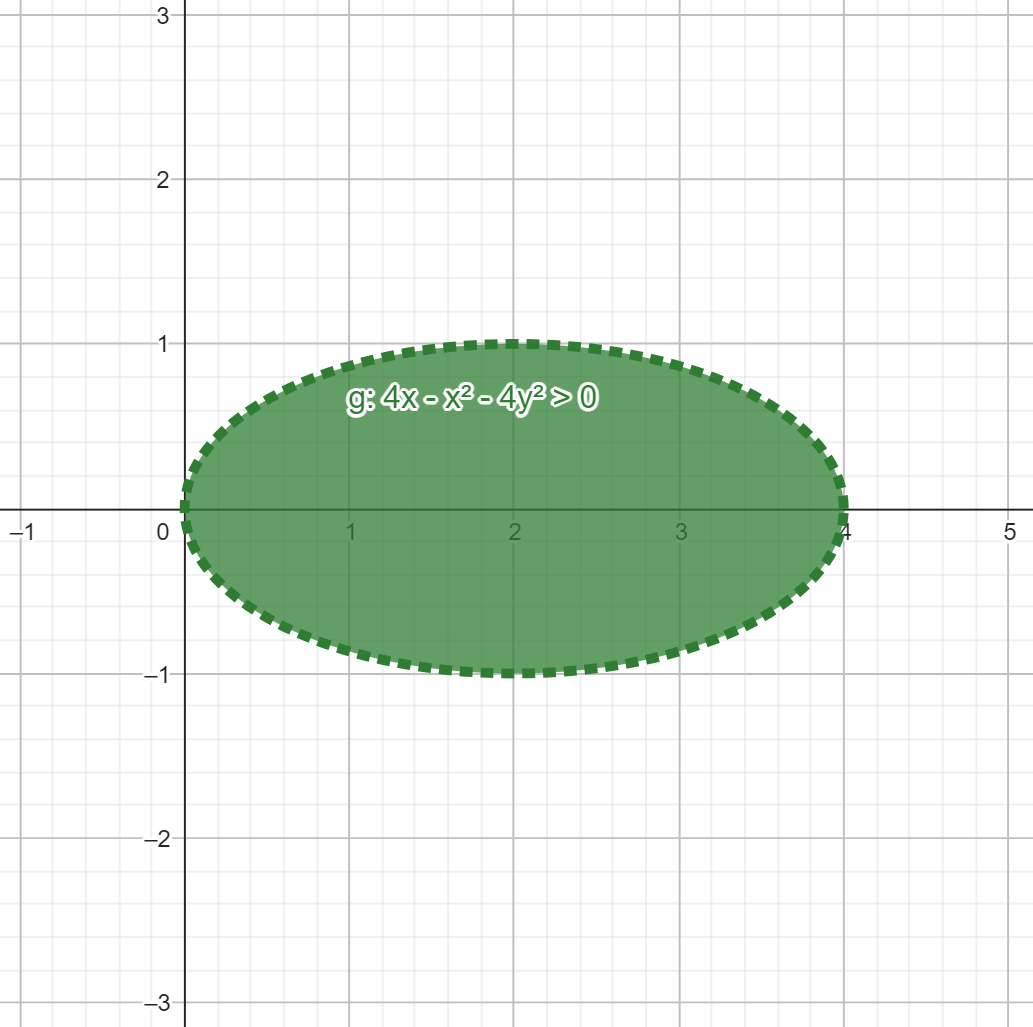
\includegraphics[width=.9\textwidth]{img/grafico-ex3-1.png}
		\caption*{Grafico $4x-x^{2}-4y^{2} > 0$.}
	\end{figure}\newpage

	\begin{figure}[!htp]
		\centering
		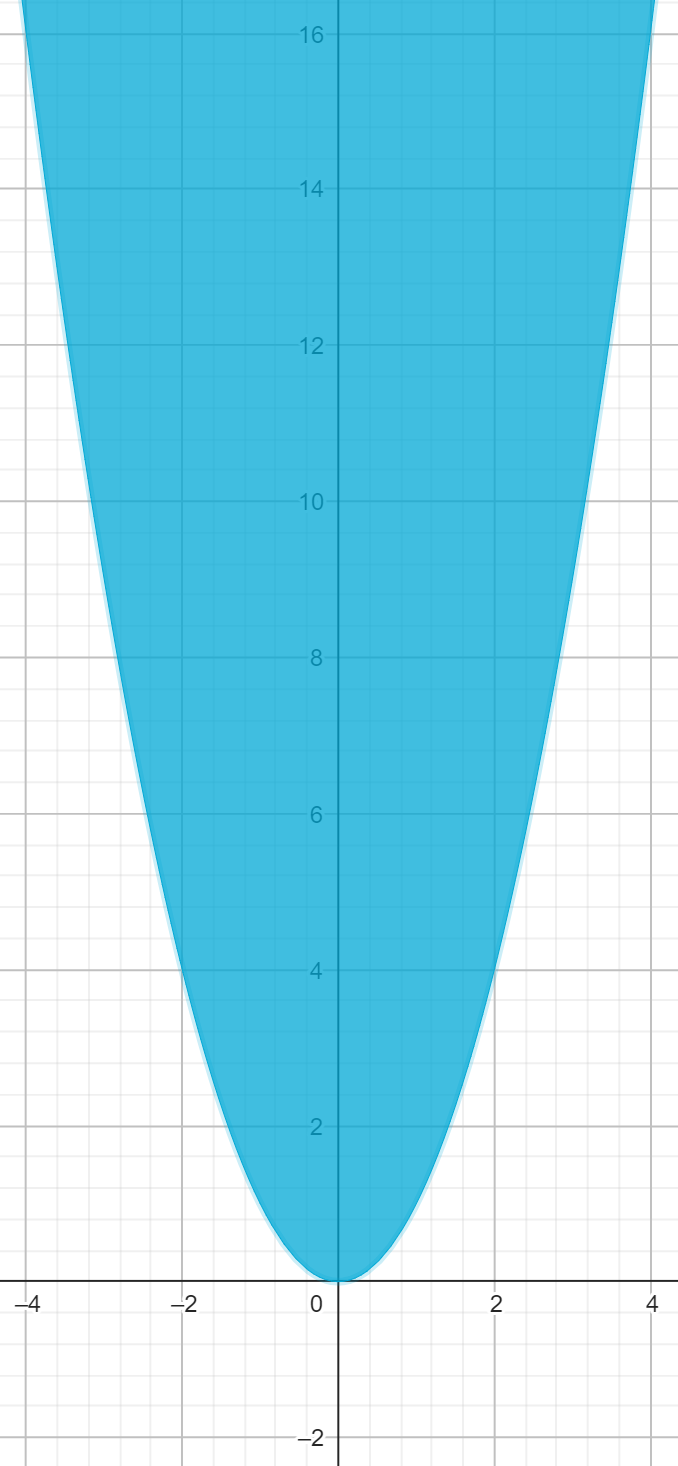
\includegraphics[width=.6\textwidth]{img/grafico-ex3-2.png}
		\caption*{Grafico $y-x^{2} \ge 0$.}
	\end{figure}\newpage
	
	\begin{figure}[!htp]
		\centering
		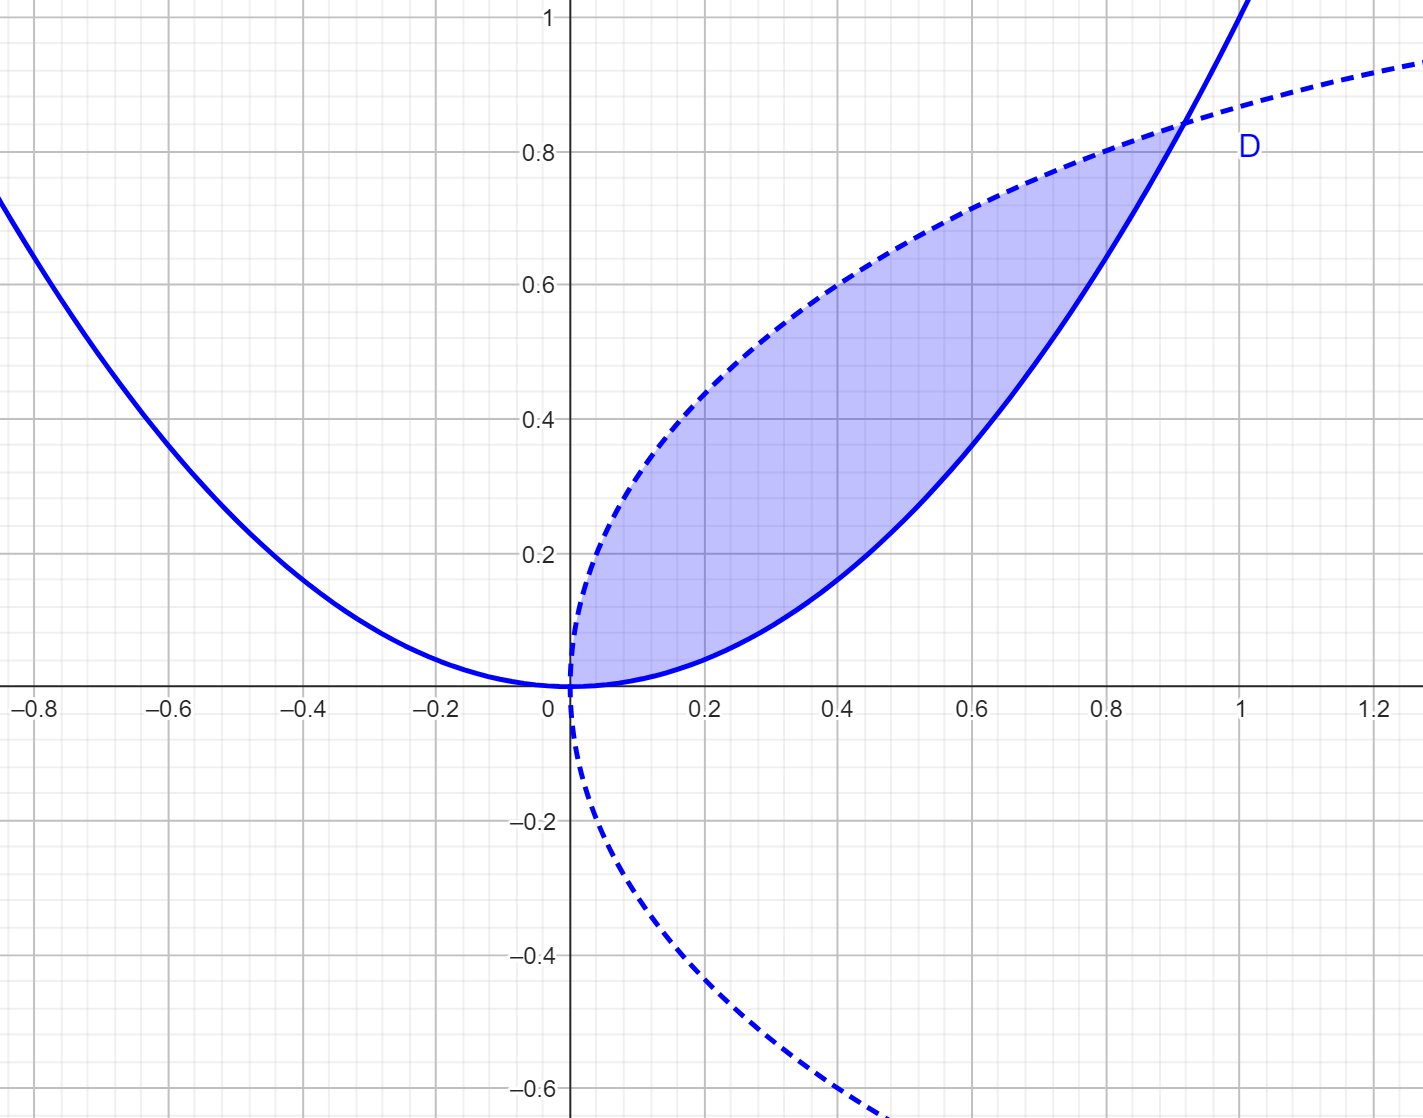
\includegraphics[width=\textwidth]{img/grafico-ex3-3.png}
		\caption*{Grafico del dominio completo.}
	\end{figure}\newpage

	\subsubsection{Dimostrazione che un punto sia interno al dominio}

	Una richiesta banale ma che potrebbe capitare, nonostante sia molto raro, è la seguente (estratta dall'esame del 25/06/2021): \textcolor{Green4}{\textbf{\emph{Sia $D\subset\mathbb{R}^{2}$ il dominio naturale della funzione:}}
	\begin{equation*}
		f\left(x,y\right) = \sqrt{y-x^{2}}-\ln\left(4x-x^{2}-4y^{2}\right)
	\end{equation*}
	\textbf{\emph{Si dimostri che il punto $P\left(\frac{1}{2}, \frac{1}{2}\right)$ è interno all'insieme $D$.}}}\newline

	\noindent
	Il \textbf{primo passo} è prendere le disuguaglianze del dominio e considerarle in modo stretto, ovvero:
	\begin{equation*}
		\begin{array}{lcl}
			y-x^{2} \ge 0			& \longrightarrow & y-x^{2} > 0 \\
			4x - x^{2} - 4y^{2} > 0	& \longrightarrow & 4x - x^{2} - 4y^{2} > 0
		\end{array}
	\end{equation*}
	Il \textbf{secondo passo} è sostituire i valori del punto dato dall'esercizio e verificare la veridicità delle disuguaglianze. In questo caso, si sostituisce il punto $P\left(\frac{1}{2}, \frac{1}{2}\right)$ all'interno delle due disuguaglianze:
	\begin{equation*}
		\begin{array}{lcl}
			y -x^{2} > 0			& \longrightarrow & \dfrac{1}{2} - \dfrac{1^{2}}{2^{2}} > 0 \Longrightarrow \dfrac{1}{4} > 0 \hspace{1em} \textcolor{Green4}{\checkmark} \\ [1em]
			4x - x^{2} - 4y^{2} > 0	& \longrightarrow & 4 \cdot \dfrac{1}{2} - \dfrac{1^{2}}{2^{2}} - 4 \cdot \dfrac{1^{2}}{2^{2}} > 0 \Longrightarrow \dfrac{3}{4} > 0 \hspace{1em} \textcolor{Green4}{\checkmark}
		\end{array}
	\end{equation*}
	Il punto $P$ rispetta entrambe le disuguaglianze, quindi è un punto interno al dominio.\newpage

	\subsubsection{Direzione della funzione affinché essa sia di massima crescita}\label{par: direzione della funzione affinché essa sia di massima crescita}

	Una richiesta che si può trovare negli esami ma non è tra le più richieste, è la seguente: \textcolor{Green4}{\textbf{\emph{Sia $D\subset\mathbb{R}^{2}$ il dominio naturale della funzione:}}
	\begin{equation*}
		f\left(x,y\right) = \sqrt{y-x^{2}}-\ln\left(4x-x^{2}-4y^{2}\right)
	\end{equation*}
	\textbf{\emph{In quale direzione ci si deve muovere da $P$ per garantire a $f$ la massima crescita?}}}\newline

	\noindent
	La direzione $\overrightarrow{v}$ di massima crescita è quella del gradiente di $f$ nel punto $P$. Per cui, per calcolare il gradiente sono necessari due passaggi fondamentali. Il \textbf{primo passo} è calcolare la derivata parziale rispetto a $x$:
	\begin{equation*}
		\begin{array}{rcl}
			f\left(x,y\right) &=& \sqrt{y-x^{2}}-\ln\left(4x-x^{2}-4y^{2}\right) \\ [1em]
			f\left(x,y\right) &=& \dfrac{\partial}{\partial x}\left( \sqrt{y-x^{2}}-\ln\left(4x-x^{2}-4y^{2}\right) \right) \\ [1.5em]
			&\downarrow& \text{si utilizza la regola } \frac{\partial}{\partial x}\left(f+g\right) = \frac{\partial}{\partial x}\left(f\right) + \frac{\partial}{\partial x}\left(g\right) \\ [1em]
			f\left(x,y\right) &=& \dfrac{\partial}{\partial x}\left( \sqrt{y-x^{2}}\right)- \dfrac{\partial}{\partial x}\left(\ln\left(4x-x^{2}-4y^{2}\right) \right) \\ [1.5em]
			&\downarrow& \text{derivata della radice quadrata per la derivata dell'argomento} \\ [1em]
			f\left(x,y\right) &=& \dfrac{1}{2\sqrt{y-x^{2}}}\cdot\left(-2x\right) - \dfrac{\partial}{\partial x}\left(\ln\left(4x-x^{2}-4y^{2}\right) \right) \\ [1.5em]
			&\downarrow& \text{derivata del logaritmo per la derivata dell'argomento} \\ [1em]
			f\left(x,y\right) &=& \dfrac{1}{2\sqrt{y-x^{2}}}\cdot\left(-2x\right) - \dfrac{1}{4x-x^{2}-4y^{2}} \cdot \left(4-2x\right) \\ [1.5em]
			&\downarrow& \text{semplificazioni} \\ [1em]
			\dfrac{\partial f}{\partial x}\left(x,y\right) &=& -\dfrac{x}{\sqrt{y-x^{2}}} - \dfrac{4-2x}{4x-x^{2}-4y^{2}} \\ [1.5em]
		\end{array}
	\end{equation*}\newpage

	\noindent
	Il \textbf{secondo passo} è calcolare la derivata parziale rispetto a $y$:
	\begin{equation*}
		\begin{array}{rcl}
			f\left(x,y\right) &=& \sqrt{y-x^{2}}-\ln\left(4x-x^{2}-4y^{2}\right) \\ [1em]
			f\left(x,y\right) &=& \dfrac{\partial}{\partial y}\left( \sqrt{y-x^{2}}-\ln\left(4x-x^{2}-4y^{2}\right) \right) \\ [1.5em]
			&\downarrow& \text{si utilizza la regola } \frac{\partial}{\partial y}\left(f+g\right) = \frac{\partial}{\partial y}\left(f\right) + \frac{\partial}{\partial y}\left(g\right) \\ [1em]
			f\left(x,y\right) &=& \dfrac{\partial}{\partial y}\left( \sqrt{y-x^{2}}\right) - \dfrac{\partial}{\partial y}\left(\ln\left(4x-x^{2}-4y^{2}\right) \right) \\ [1.5em]
			&\downarrow& \text{derivata della radice quadrata per la derivata dell'argomento} \\ [1em]
			f\left(x,y\right) &=& \dfrac{1}{2\sqrt{y-x^{2}}}\cdot\left(1\right) - \dfrac{\partial}{\partial y}\left(\ln\left(4x-x^{2}-4y^{2}\right) \right) \\ [1.5em]
			&\downarrow& \text{derivata del logaritmo per la derivata dell'argomento} \\ [1em]
			\dfrac{\partial f}{\partial y} \left(x,y\right) &=& \dfrac{1}{2\sqrt{y-x^{2}}} - \dfrac{1}{4x-x^{2}-4y^{2}}\cdot\left(-8y\right) \\ [1.5em]
			\dfrac{\partial f}{\partial y} \left(x,y\right) &=& \dfrac{1}{2\sqrt{y-x^{2}}} + \dfrac{8y}{4x-x^{2}-4y^{2}}
		\end{array}
	\end{equation*}\newpage

	\noindent
	Il \textbf{terzo passo} è quello di andare a sostituire i valori del punto $P$ all'interno delle derivate parziali. Così facendo, si troverà la direzione di massima crescita, ovvero il gradiente:
	\begin{equation*}
		\begin{array}{rcl}
			\dfrac{\partial f}{\partial x}\left(x,y\right) &=& -\dfrac{x}{\sqrt{y-x^{2}}} - \dfrac{4-2x}{4x-x^{2}-4y^{2}} \\ [1.5em]
			\dfrac{\partial f}{\partial x}\left(\dfrac{1}{2},\dfrac{1}{2}\right) &=& -\dfrac{\dfrac{1}{2}}{\sqrt{\dfrac{1}{2}-\dfrac{1^{2}}{2^{2}}}} - \dfrac{4-2 \cdot \dfrac{1}{2}}{4 \cdot \dfrac{1}{2} - \dfrac{1^{2}}{2^{2}} -4 \cdot \dfrac{1^{2}}{2^{2}}} \\ [3em]
			\dfrac{\partial f}{\partial x}\left(\dfrac{1}{2},\dfrac{1}{2}\right) &=& -1 - \dfrac{3}{2 - \dfrac{1}{4} - 1} \\ [1.5em]
			\dfrac{\partial f}{\partial x}\left(\dfrac{1}{2},\dfrac{1}{2}\right) &=& -5 \\ [3em]
			\dfrac{\partial f}{\partial y}\left(x,y\right) &=& \dfrac{1}{2\sqrt{y-x^{2}}} + \dfrac{8y}{4x-x^{2}-4y^{2}} \\ [1.5em]
			\dfrac{\partial f}{\partial y}\left(\dfrac{1}{2},\dfrac{1}{2}\right) &=& \dfrac{1}{2\sqrt{\dfrac{1}{2} - \dfrac{1^{2}}{2^{2}}}} + \dfrac{8 \cdot \dfrac{1}{2}}{4 \cdot \dfrac{1}{2} - \dfrac{1^{2}}{2^{2}} - 4 \cdot \dfrac{1^{2}}{2^{2}}} \\ [3em]
			\dfrac{\partial f}{\partial y}\left(\dfrac{1}{2},\dfrac{1}{2}\right) &=& 1 + \dfrac{4}{2 - \dfrac{1}{4} - 1} \\ [1.5em]
			\dfrac{\partial f}{\partial y}\left(\dfrac{1}{2},\dfrac{1}{2}\right) &=& \dfrac{19}{3}
		\end{array}
	\end{equation*}
	Si conclude l'esercizio:
	\begin{equation*}
		\overrightarrow{v} = \nabla f\left(P\right) = \left(-5, \dfrac{19}{3}\right)
	\end{equation*}\newpage

	\subsubsection{Specificare se un dominio è aperto/chiuso, limitato/illimitato, connesso/sconnesso, compatto}

	Questa richiesta è molto probabile che ci sia all'esame. Solitamente, viene accoppiata con la scrittura del dominio e della sua rappresentazione (pagina \pageref{par: rappresentare la funzione nel piano cartesiano}). Un esempio di tema d'esame (03/03/2023): \textcolor{Green4}{\textbf{\emph{Data la funzione:}}
	\begin{equation*}
		f\left(x,y\right) = y e^{\sqrt{x-2y}} - \ln\left(xy\right)
	\end{equation*}
	\textbf{\emph{Determinare analiticamente il suo dominio naturale $D$ e poi rappresentarlo nel piano cartesiano. Stabilire se $D$ è un insieme limitato/illimitato, aperto/chiuso, connesso/sconnesso (motivare le risposte!).}}}\newline

	\noindent
	Prima di tutto si stabilisce il dominio:
	\begin{equation*}
		D = \left\{\left(x,y\right) \in \mathbb{R}^{2} \: : \: \left(x-2y \ge 0\right) \land \left(xy > 0\right)\right\}
	\end{equation*}
	Ovvero si impone le condizioni di esistenza sulla radice quadrata e il logaritmo. La sua rappresentazione grafica:
	\begin{figure}[!htp]
		\centering
		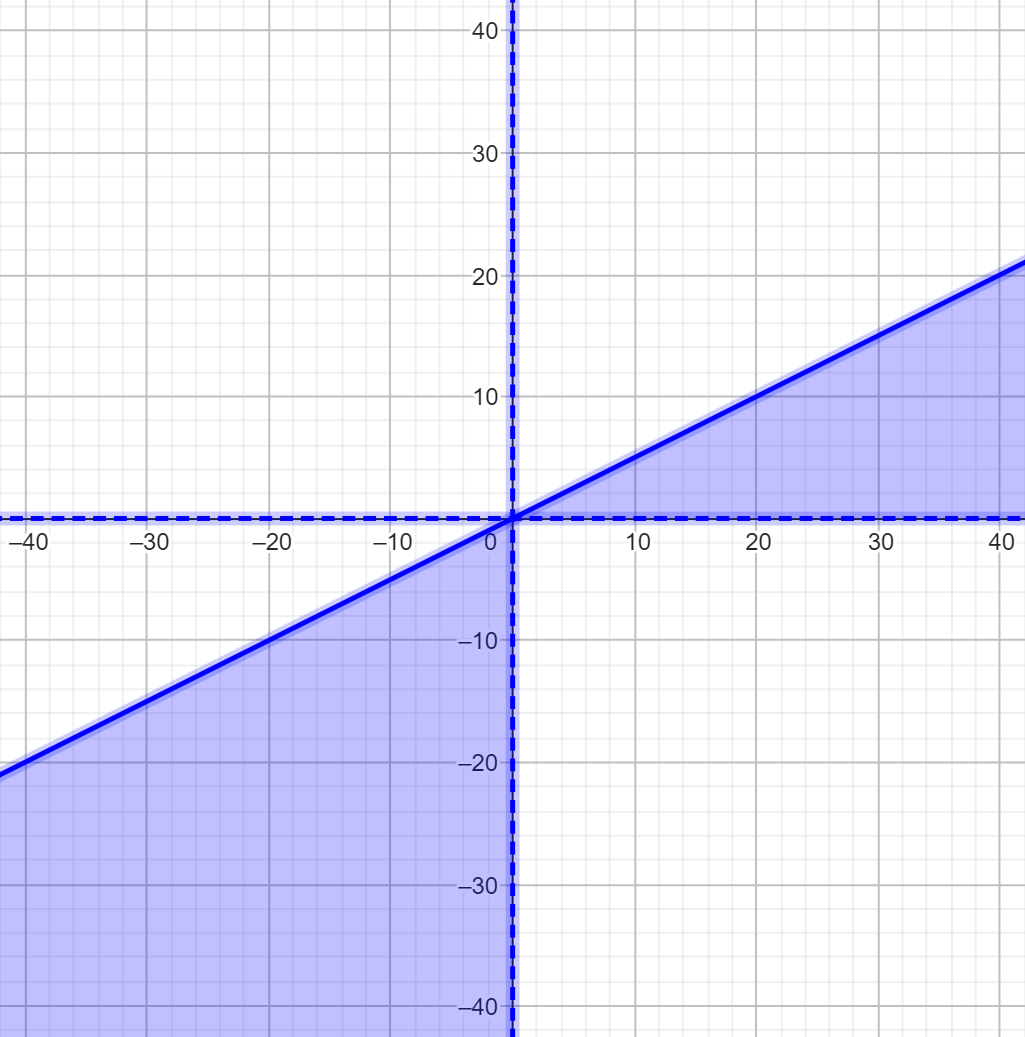
\includegraphics[width=.8\textwidth]{img/grafico-ex3-4.png}
	\end{figure}
	\begin{itemize}
		\item \textbf{Limitato o illimitato?} Il dominio è illimitato, dato che continua all'infinito, ovvero non esiste una palla con centro l'origine e raggio $r \in \mathbb{R}$ che contiene $D$.
		
		\item \textbf{Aperto o chiuso?} Il dominio non è né chiuso né aperto poiché contiene alcuni punti della sua frontiera ma non tutti.
		
		\item \textbf{Connesso o sconnesso?} Il dominio è sconnesso poiché non è connesso per archi. Infatti, come si può vedere dal grafico del dominio, quest'ultimo è l'unione di due insiemi.
	\end{itemize}
	Nell'esame del 07/02/2023, la funzione di riferimento e il dominio erano:
	\begin{equation*}
		\begin{array}{rcl}
			f\left(x,y\right) &=& y + \dfrac{1}{\sqrt{1 - \ln\left(y-x^{2}\right)}} - \ln\left(x\right) \\ [1.5em]
			D &=& \left\{\left(x,y\right) \in \mathbb{R}^{2} \: : \: \left(y > x^{2}\right) \land \left(y < x^{2} + e\right) \land \left(x > 0\right)\right\}
		\end{array}
	\end{equation*}
	\begin{figure}[!htp]
		\centering
		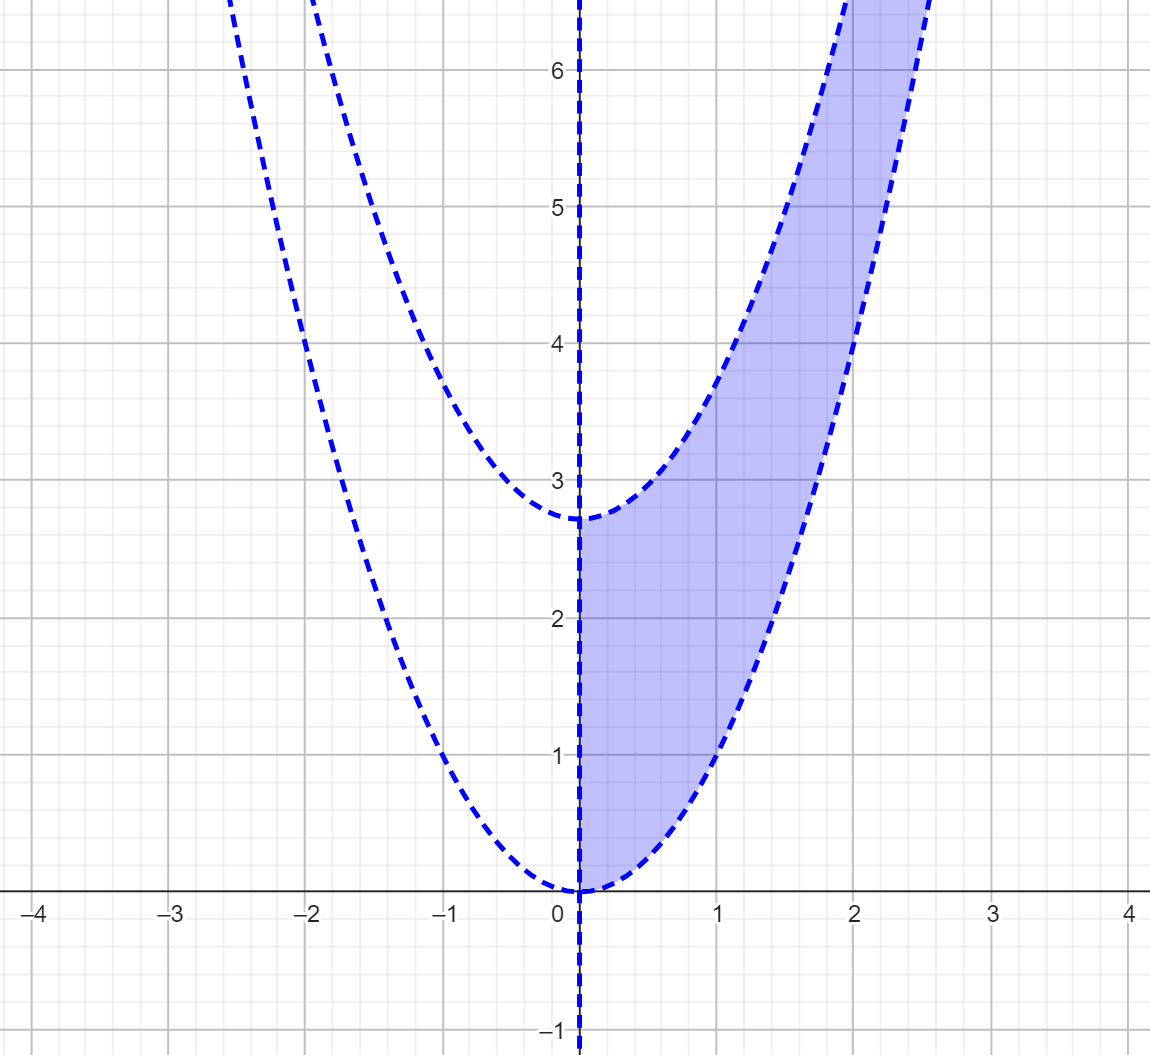
\includegraphics[width=\textwidth]{img/grafico-ex3-5.png}
		\caption*{Dominio della funzione.}
	\end{figure}

	\noindent
	In questo caso, il dominio è illimitato per lo stesso motivo dell'esercizio precedente; il dominio è aperto poiché tutti i punti sono interni e inoltre è connesso per archi.\newpage

	\subsubsection{Trovare l'equazione al piano tangente}\label{par: trovare l'equazione al piano tangente}

	Uno degli esercizi più richiesti insieme alla derivata direzionale, è quello di trovare l'equazione al piano tangente. Si prenda in considerazione il tema d'esame del 07/02/2023 in cui veniva chiesto: \textcolor{Green4}{\textbf{\emph{Data la funzione:}}
	\begin{equation*}
		f\left(x,y\right) = y + \dfrac{1}{\sqrt{1 - \ln\left(y - x^{2}\right)}} - \ln\left(x\right)
	\end{equation*}
	\textbf{\emph{Scrivere l'equazione del piano tangente al grafico di $f$ nel punto $\left(1, 2, f\left(1,2\right)\right)$.}}}\newline

	\noindent
	Anche in questo caso, come accadeva nel caso in cui si doveva trovare la direzione della funzione affinché essa sia di massima crescita (pagina \pageref{par: direzione della funzione affinché essa sia di massima crescita}), è necessario calcolare le derivate parziali di $f\left(x,y\right)$. Quindi, il \textbf{primo passo} è calcolare la derivata parziale rispetto a $x$:
	\begin{equation*}
		\begin{array}{rcl}
			f\left(x,y\right) &=& y + \dfrac{1}{\sqrt{1 - \ln\left(y - x^{2}\right)}} - \ln\left(x\right) \\ [1.5em]
			f\left(x,y\right) &=& \dfrac{\partial}{\partial x} \left( y + \dfrac{1}{\sqrt{1 - \ln\left(y - x^{2}\right)}} - \ln\left(x\right) \right) \\ [2em]
			&\downarrow& \text{si utilizza la regola } \frac{\partial}{\partial x}\left(f+g\right) = \frac{\partial}{\partial x}\left(f\right) + \frac{\partial}{\partial x}\left(g\right) \\ [1em]
			f\left(x,y\right) &=& \dfrac{\partial}{\partial x} \left(y\right) + \dfrac{\partial}{\partial x} \left(\dfrac{1}{\sqrt{1 - \ln\left(y - x^{2}\right)}}\right) - \dfrac{\partial}{\partial x}\left(\ln\left(x\right)\right) \\ [1.5em]
			&\downarrow& \text{si utilizza la regola } \frac{\partial}{\partial x}\left(\frac{1}{f}\right) = -\frac{\frac{\partial}{\partial x}\left(f\right)}{f^{2}} \\ [1em]
			\dfrac{\partial f}{\partial x}\left(x,y\right) &=& 0 - \dfrac{\dfrac{1}{2\sqrt{1-\ln\left(y-x^{2}\right)}} \cdot \left(-\dfrac{1}{y-x^{2}} \cdot \left(-2x\right)\right)}{\sqrt{1 - \ln\left(y - x^{2}\right)}^{2}} - \left(\dfrac{1}{x} \cdot \left(1\right)\right) \\ [2em]
			\dfrac{\partial f}{\partial x}\left(x,y\right) &=& -\dfrac{\dfrac{1}{2\sqrt{1-\ln\left(y-x^{2}\right)}} \cdot \left(\dfrac{2x}{y-x^{2}}\right)}{1 - \ln\left(y - x^{2}\right)} - \dfrac{1}{x} \\ [2em]
			\dfrac{\partial f}{\partial x}\left(x,y\right) &=& -\dfrac{\dfrac{x}{\sqrt{1-\ln\left(y-x^{2}\right)} \cdot \left(y-x^{2}\right)}}{1-\ln\left(y-x^{2}\right)} - \dfrac{1}{x} \\ [2em]
			\dfrac{\partial f}{\partial x}\left(x,y\right) &=& -\dfrac{x}{\sqrt{1 - \ln\left(y-x^{2}\right)} \cdot \left(y-x^{2}\right) \cdot \left(1 - \ln\left(y-x^{2}\right)\right)} - \dfrac{1}{x}
		\end{array}
	\end{equation*}\newpage

	\nointerlineskip
	Il \textbf{secondo passo} è calcolare la derivata parziale rispetto a $y$:
	\begin{equation*}
		\begin{array}{rcl}
			f\left(x,y\right) &=& y + \dfrac{1}{\sqrt{1 - \ln\left(y - x^{2}\right)}} - \ln\left(x\right) \\ [1.5em]
			f\left(x,y\right) &=& \dfrac{\partial}{\partial y} \left( y + \dfrac{1}{\sqrt{1 - \ln\left(y - x^{2}\right)}} - \ln\left(x\right) \right) \\ [2em]
			&\downarrow& \text{si utilizza la regola } \frac{\partial}{\partial y}\left(f+g\right) = \frac{\partial}{\partial y}\left(f\right) + \frac{\partial}{\partial y}\left(g\right) \\ [1em]
			f\left(x,y\right) &=& \dfrac{\partial}{\partial y} \left(y\right) + \dfrac{\partial}{\partial y} \left(\dfrac{1}{\sqrt{1 - \ln\left(y - x^{2}\right)}}\right) - \dfrac{\partial}{\partial y}\left(\ln\left(x\right)\right) \\ [1.5em]
			&\downarrow& \text{si utilizza la regola } \frac{\partial}{\partial y}\left(\frac{1}{f}\right) = -\frac{\frac{\partial}{\partial y}\left(f\right)}{f^{2}} \\ [1em]
			\dfrac{\partial f}{\partial y}\left(x,y\right) &=& 1 - \dfrac{\dfrac{1}{2\sqrt{1-\ln\left(y-x^{2}\right)}} \cdot \left(-\dfrac{1}{y-x^{2}} \cdot 1\right)}{\sqrt{1-\ln\left(y-x^{2}\right)}^{2}} - 0 \\ [2em]
			\dfrac{\partial f}{\partial y}\left(x,y\right) &=& 1 + \dfrac{1}{2\sqrt{1-\ln\left(y-x^{2}\right)} \cdot \left(y-x^{2}\right) \cdot \left(1-\ln\left(y-x^{2}\right)\right)}
		\end{array}
	\end{equation*}
	Il \textbf{terzo passo} è scrivere il gradiente valutato nel punto dato, ovvero in $P\left(1,2\right)$. Quindi, si prendono le derivate parziali trovate, si sostituiscono i valori e si utilizzano nel gradiente:
	\begin{equation*}
		\begin{array}{rcl}
			\dfrac{\partial f}{\partial x}\left(x,y\right) &=& -\dfrac{x}{\sqrt{1 - \ln\left(y-x^{2}\right)} \cdot \left(y-x^{2}\right) \cdot \left(1 - \ln\left(y-x^{2}\right)\right)} - \dfrac{1}{x} \\ [1.5em]
			\dfrac{\partial f}{\partial x}\left(1,2\right) &=& -\dfrac{1}{\sqrt{1 - \ln\left(2-1^{2}\right)} \cdot \left(2-1^{2}\right) \cdot \left(1 - \ln\left(2-1^{2}\right)\right)} - \dfrac{1}{1} \\ [1.5em]
			\dfrac{\partial f}{\partial x}\left(1,2\right) &=& -\dfrac{1}{\sqrt{1 - \ln\left(1\right)} \cdot 1 \cdot \left(1 - \ln\left(1\right)\right)} - 1 \\ [1.5em]
			\dfrac{\partial f}{\partial x}\left(1,2\right) &=& -\dfrac{1}{1 \cdot 1 \cdot 1} - 1 \\ [1.5em]
			\dfrac{\partial f}{\partial x}\left(1,2\right) &=& -2 \\ [2em]
			\dfrac{\partial f}{\partial y}\left(x,y\right) &=& 1 + \dfrac{1}{2\sqrt{1-\ln\left(y-x^{2}\right)} \cdot \left(y-x^{2}\right) \cdot \left(1-\ln\left(y-x^{2}\right)\right)} \\ [1.5em]
			\dfrac{\partial f}{\partial y}\left(1,2\right) &=& 1 + \dfrac{1}{2\sqrt{1-\ln\left(2-1^{2}\right)} \cdot \left(2-1^{2}\right) \cdot \left(1-\ln\left(2-1^{2}\right)\right)} \\ [1.5em]
			\dfrac{\partial f}{\partial y}\left(1,2\right) &=& 1 + \dfrac{1}{2 \cdot 1 \cdot 1 \cdot 1} \\ [1.5em]
			\dfrac{\partial f}{\partial y}\left(1,2\right) &=& \dfrac{3}{2}
		\end{array}
	\end{equation*}\newpage

	\noindent
	Per cui il gradiente corrisponde al valore:
	\begin{equation*}
		\nabla f\left(P\right) = \nabla f\left(1,2\right) = \left(-2, \dfrac{3}{2}\right)
	\end{equation*}
	Il \textbf{quarto e ultimo passo} è scrivere l'equazione del piano tangente. Il piano tangente nel punto $\left(x,y,\left(x_{0}, y_{0}\right)\right)$ è rappresentato dall'equazione:
	\begin{equation*}
		z = f\left(x_{0},y_{0}\right) + \dfrac{\partial f}{\partial x}\left(x_{0}, y_{0}\right)\left(x-x_{0}\right) + \dfrac{\partial f}{\partial y}\left(x_{0}, y_{0}\right)\left(y-y_{0}\right)
	\end{equation*}
	Dove $f\left(x,y\right)$ è la funzione e $\left(x_{0},y_{0}\right)$ è il punto in cui è differenziabile.

	Grazie a questo richiamo di teoria, adesso è possibile scrivere l'equazione del piano tangente. Quindi, si prende il punto differenziabile, cioè $P\left(1,2\right)$, e si sostituisce nell'equazione iniziale:
	\begin{equation*}
		\begin{array}{rcl}
			f\left(x,y\right) &=& y + \dfrac{1}{\sqrt{1 - \ln\left(y - x^{2}\right)}} - \ln\left(x\right) \\ [1.5em]
			f\left(1,2\right) &=& 2 + \dfrac{1}{\sqrt{1 - \ln\left(2 - 1^{2}\right)}} - \ln\left(1\right) \\ [1.5em]
			f\left(1,2\right) &=& 2 + \dfrac{1}{1} - 0 \\ [1.5em]
			f\left(1,2\right) &=& 3
		\end{array}
	\end{equation*}
	E infine si sostituiscono i valori calcolati nell'equazione del piano tangente:
	\begin{equation*}
		z = 3 - 2\left(x - 1\right) + \dfrac{3}{2}\left(y-2\right) = 3 - 2x +2 + \dfrac{3}{2}y - 3 = -2x + \dfrac{3}{2}y + 2
	\end{equation*}\newpage

	\subsubsection{Calcolare il gradiente della funzione ($\nabla f$)}\label{par: calcolare il gradiente della funzione}

	Esercizio difficile che venga richiesto, ma una volta è capitato, è la richiesta esplicita di calcolare il gradiente. Solitamente viene richiesto di trovare la massima crescita della funzione, cioè il gradiente, o la derivata direzionale. In questo caso, si calcola direttamente il gradiente come è stato fatto nei precedenti capitoli. Si riporta comunque i passaggi da eseguire. Si faccia riferimento al testo d'esame del 15/09/2021, gruppo A: \textcolor{Green4}{\textbf{\emph{Data la funzione:}}
	\begin{equation*}
		f\left(x,y\right) = \log\left(x^{2} - 4x + 4y^{2}\right) - \sqrt{2x - x^{2}}
	\end{equation*}
	\textbf{\emph{Calcolare $\nabla f\left(P\right)$, dove $P$ è il punto di coordinate $(1,2)$.}}}\newline
	
	\noindent
	Il \textbf{primo passo} è calcolare la derivata parziale rispetto $x$:
	\begin{equation*}
		\begin{array}{rcl}
			f\left(x,y\right) &=& \log\left(x^{2} - 4x + 4y^{2}\right) - \sqrt{2x - x^{2}} \\ [.5em]
			f\left(x,y\right) &=& \dfrac{\partial}{\partial x} \left(\log\left(x^{2} - 4x + 4y^{2}\right) - \sqrt{2x - x^{2}}\right) \\ [1.5em]
			f\left(x,y\right) &=& \dfrac{\partial}{\partial x}\left(\log\left(x^{2}-4x+4y^{2}\right)\right) - \dfrac{\partial}{\partial x}\left(\sqrt{2x-x^{2}}\right) \\ [1.5em]
			\dfrac{\partial f}{\partial x}\left(x,y\right) &=& \dfrac{1}{x^{2}-4x+4y^{2}} \cdot \left(2x - 4\right) - \dfrac{1}{2\sqrt{2x-x^{2}}} \cdot \left(2-2x\right) \\ [1.5em]
			\dfrac{\partial f}{\partial x}\left(x,y\right) &=& \dfrac{2x - 4}{x^{2}-4x+4y^{2}} - \dfrac{2-2x}{2\sqrt{2x-x^{2}}}
		\end{array}
	\end{equation*}
	Il \textbf{secondo passo} è calcolare la derivata parziale rispetto $y$:
	\begin{equation*}
		\begin{array}{rcl}
			f\left(x,y\right) &=& \log\left(x^{2} - 4x + 4y^{2}\right) - \sqrt{2x - x^{2}} \\ [.5em]
			f\left(x,y\right) &=& \dfrac{\partial}{\partial y} \left(\log\left(x^{2} - 4x + 4y^{2}\right) - \sqrt{2x - x^{2}}\right) \\ [1.5em]
			f\left(x,y\right) &=& \dfrac{\partial}{\partial y}\left(\log\left(x^{2}-4x+4y^{2}\right)\right) - \dfrac{\partial}{\partial y}\left(\sqrt{2x-x^{2}}\right) \\ [1.5em]
			\dfrac{\partial f}{\partial y}\left(x,y\right) &=& \dfrac{1}{x^{2}-4x+4y^{2}} \cdot \left(8y\right) - \dfrac{1}{2\sqrt{2x-x^{2}}} \cdot \left(0\right) \\ [1.5em]
			\dfrac{\partial f}{\partial y}\left(x,y\right) &=& \dfrac{8y}{x^{2} - 4x + 4y^{2}}
		\end{array}
	\end{equation*}
	Il \textbf{terzo passo} è sostituire il punto di coordinate $P\left(1,2\right)$ all'interno delle derivate parziali e calcolare il gradiente:
	\begin{equation*}
		\begin{array}{rcl}
			\dfrac{\partial f}{\partial x}\left(x,y\right) &=& \dfrac{2x - 4}{x^{2}-4x+4y^{2}} - \dfrac{2-2x}{2\sqrt{2x-x^{2}}} \\ [1.5em]
			\dfrac{\partial f}{\partial x}\left(1,2\right) &=& \dfrac{2 \cdot 1 - 4}{1^{2}-4 \cdot 1+4 \cdot 2^{2}} - \dfrac{2-2 \cdot 1}{2\sqrt{2 \cdot 1- 1^{2}}} \\ [1.5em]
			\dfrac{\partial f}{\partial x}\left(1,2\right) &=& -\dfrac{2}{13} - \dfrac{0}{2} = -\dfrac{2}{13}
		\end{array}
	\end{equation*}\newpage
	\begin{equation*}
		\begin{array}{rcl}
			\dfrac{\partial f}{\partial y}\left(x,y\right) &=& \dfrac{8y}{x^{2} - 4x + 4y^{2}} \\ [1.5em]
			\dfrac{\partial f}{\partial y}\left(1,2\right) &=& \dfrac{8 \cdot 2}{1^{2} - 4 \cdot 1 + 4 \cdot 2^{2}} \\ [1.5em]
			\dfrac{\partial f}{\partial y}\left(1,2\right) &=& \dfrac{16}{13}
		\end{array}
	\end{equation*}
	Il gradiente dunque corrisponde a:
	\begin{equation*}
		\nabla f\left(P\right) = \nabla f\left(1,2\right) = \left(-\dfrac{2}{13}, \dfrac{16}{13}\right)
	\end{equation*}\newpage

	\subsubsection{Calcolare la derivata direzionale}

	Un esercizio richiestissimo, è il calcolo della derivata direzionale. Un esercizio tipo è il seguente, estratto dall'esame del 15/09/2021, gruppo A: \textcolor{Green4}{\textbf{\emph{Data la funzione:}}
	\begin{equation*}
		f\left(x,y\right) = \log\left(x^{2} -4x + 4y^{2}\right) - \sqrt{2x - x^{2}}
	\end{equation*}
	\textbf{\emph{Calcolare la derivata direzionale di $f$ in $P$ rispetto al versore $\overrightarrow{v} = \left(\frac{\sqrt{3}}{2}, \frac{1}{2}\right)$.}}}\newline

	\noindent
	La derivata direzionale di una funzione in un punto rispetto ad un versore, non è altro che la moltiplicazione del gradiente della funzione in quel punto per il versore, ovvero:
	\begin{equation*}
		\nabla f\left(P\right) \cdot \overrightarrow{v}
	\end{equation*}
	Viene da sé che è necessario prima calcolare il gradiente e poi calcolare il versore. Come \textbf{primo passo} si calcolano le derivate parziali:
	\begin{equation*}
		\begin{array}{rcl}
			f\left(x,y\right) &=& \log\left(x^{2} - 4x + 4y^{2}\right) - \sqrt{2x - x^{2}} \\ [.5em]
			f\left(x,y\right) &=& \dfrac{\partial}{\partial x} \left(\log\left(x^{2} - 4x + 4y^{2}\right) - \sqrt{2x - x^{2}}\right) \\ [1.5em]
			f\left(x,y\right) &=& \dfrac{\partial}{\partial x}\left(\log\left(x^{2}-4x+4y^{2}\right)\right) - \dfrac{\partial}{\partial x}\left(\sqrt{2x-x^{2}}\right) \\ [1.5em]
			\dfrac{\partial f}{\partial x}\left(x,y\right) &=& \dfrac{1}{x^{2}-4x+4y^{2}} \cdot \left(2x - 4\right) - \dfrac{1}{2\sqrt{2x-x^{2}}} \cdot \left(2-2x\right) \\ [1.5em]
			\dfrac{\partial f}{\partial x}\left(x,y\right) &=& \dfrac{2x - 4}{x^{2}-4x+4y^{2}} - \dfrac{2-2x}{2\sqrt{2x-x^{2}}} \\ [3em]
			%
			f\left(x,y\right) &=& \log\left(x^{2} - 4x + 4y^{2}\right) - \sqrt{2x - x^{2}} \\ [.5em]
			f\left(x,y\right) &=& \dfrac{\partial}{\partial y} \left(\log\left(x^{2} - 4x + 4y^{2}\right) - \sqrt{2x - x^{2}}\right) \\ [1.5em]
			f\left(x,y\right) &=& \dfrac{\partial}{\partial y}\left(\log\left(x^{2}-4x+4y^{2}\right)\right) - \dfrac{\partial}{\partial y}\left(\sqrt{2x-x^{2}}\right) \\ [1.5em]
			\dfrac{\partial f}{\partial y}\left(x,y\right) &=& \dfrac{1}{x^{2}-4x+4y^{2}} \cdot \left(8y\right) - \dfrac{1}{2\sqrt{2x-x^{2}}} \cdot \left(0\right) \\ [1.5em]
			\dfrac{\partial f}{\partial y}\left(x,y\right) &=& \dfrac{8y}{x^{2} - 4x + 4y^{2}}
		\end{array}
	\end{equation*}
	(calcoli già eseguiti nel paragrafo precedente, li riportiamo per convenienza)\newpage
	
	\noindent
	Il \textbf{secondo passo} è sostituire il punto fornito $P\left(1,2\right)$ all'interno delle derivate parziali così da ottenere il gradiente:
	\begin{equation*}
		\begin{array}{rcl}
			\dfrac{\partial f}{\partial x}\left(x,y\right) &=& \dfrac{2x - 4}{x^{2}-4x+4y^{2}} - \dfrac{2-2x}{2\sqrt{2x-x^{2}}} \\ [1.5em]
			\dfrac{\partial f}{\partial x}\left(1,2\right) &=& \dfrac{2 \cdot 1 - 4}{1^{2}-4 \cdot 1+4 \cdot 2^{2}} - \dfrac{2-2 \cdot 1}{2\sqrt{2 \cdot 1- 1^{2}}} \\ [1.5em]
			\dfrac{\partial f}{\partial x}\left(1,2\right) &=& -\dfrac{2}{13} - \dfrac{0}{2} = -\dfrac{2}{13} \\ [2.5em]
			%
			\dfrac{\partial f}{\partial y}\left(x,y\right) &=& \dfrac{8y}{x^{2} - 4x + 4y^{2}} \\ [1.5em]
			\dfrac{\partial f}{\partial y}\left(1,2\right) &=& \dfrac{8 \cdot 2}{1^{2} - 4 \cdot 1 + 4 \cdot 2^{2}} \\ [1.5em]
			\dfrac{\partial f}{\partial y}\left(1,2\right) &=& \dfrac{16}{13}
		\end{array}
	\end{equation*}
	Il gradiente dunque corrisponde a:
	\begin{equation*}
		\nabla f\left(P\right) = \nabla f\left(1,2\right) = \left(-\dfrac{2}{13}, \dfrac{16}{13}\right)
	\end{equation*}
	Fin qua l'esercizio è identico al calcolo del gradiente della funzione (pagina \pageref{par: calcolare il gradiente della funzione}). Il \textbf{terzo passo} è eseguire la moltiplicazione tra il versore fornito dall'esercizio $\overrightarrow{v}$ e il gradiente calcolato:
	\begin{equation*}
		\nabla f\left(P\right) \cdot \overrightarrow{v} = \left(-\dfrac{2}{13} \cdot \dfrac{\sqrt{3}}{2}, \: \dfrac{16}{13} \cdot \dfrac{1}{2}\right) = \left(-\dfrac{\sqrt{3}}{13}, \: \dfrac{8}{13}\right) = -\dfrac{\sqrt{3}}{13} + \dfrac{8}{13} = \dfrac{-\sqrt{3} + 8}{13}
	\end{equation*}\newpage

	\subsection{Alcuni esercizi d'esame svolti}\newpage

	\section{Esercizio 4 - Stabilire se una funzione è continua e parametrizzazioni}

	\subsection{Tipologie di esercizio 1}

	\subsubsection{Stabilire se una funzione è continua}

	Un \emph{evergreen} nell'esercizio 4 è la richiesta di stabilire se la funzione data è continua in un certo insieme. Il procedimento è il seguente; si estrae un esercizio dal tema d'esame del 15/09/2021, gruppo A: \textcolor{Green4}{\textbf{\emph{Stabilire se la funzione:}}
	\begin{equation*}
		f\left(x,y\right) = \begin{cases}
			\dfrac{y^{4}}{x^{2} + y^{4}} & \left(x,y\right) \ne \left(0,0\right) \\
			\\
			0	& \left(x,y\right) = \left(0,0\right)
		\end{cases}
	\end{equation*}
	\textbf{\emph{è continua in $\mathbb{R}^{2}$.}}}\newline

	\noindent
	La soluzione di questo esercizio, il più delle volte, è affermare che la funzione non è continua nell'insieme dato. Tuttavia, talvolta non è così scontato ed è necessario dimostrare il motivo della risposta.\newline
	
	\noindent
	Il \textbf{primo passo}, banale e al 90\% verificabile visivamente, è verificare che la funzione sia definita nel punto $\left(0,0\right)$. Infatti, per stabilire se la funzione è continua in $\mathbb{R}^{2}$, è \underline{necessario} che sia continua nel punto $\left(0,0\right)$.

	In questo caso, l'esercizio afferma che nel caso in cui $x$ e $y$ siano zero $\left(x,y\right) = \left(0,0\right)$, la funzione abbia risultato $0$. Per cui, la funzione è definita.\newline

	\noindent
	Il \textbf{secondo passo} è verificare che esista il limite con $x$ che tende a zero e con $y$ che tende a zero. Nel caso in cui sia $\infty$, è possibile affermare che la funzione non è continua facendo vedere i calcoli del limite. In questo caso:
	\begin{equation*}
		\begin{array}{rcl}
			\displaystyle\lim_{x \rightarrow 0} f\left(x,0\right) &=& \dfrac{0^{4}}{x^{2} + 0^{4}} = \dfrac{0}{x^{2}} = 0 \\ [1.5em]
			\displaystyle\lim_{y \rightarrow 0} f\left(0,y\right) &=& \dfrac{y^{4}}{0^{2} + y^{4}} = \dfrac{y^{4}}{y^{4}} = 1
		\end{array}
	\end{equation*}
	I limiti non coincidono, per cui è possibile affermare che la funzione non è continua nell'origine $\left(0,0\right)$, ovvero i limite di $f$ per $\left(x,y\right) \rightarrow \left(0,0\right)$ non esiste. Quindi, $f$ non è continua in $\mathbb{R}^{2}$.\newline

	\noindent
	Per completezza, si presenta un esercizio in cui una funzione è continua per capire come comportarsi. Si estrae un esercizio dal tema d'esame del 01/03/2022: \textcolor{Green4}{\textbf{\emph{Stabilire se la funzione:}}
	\begin{equation*}
		f\left(x,y\right) = \begin{cases}
			\dfrac{\left(x-1\right)\left(y-2\right)}{\sqrt{\left(x-1\right)^{2} + \left(y-2\right)^{2}}} & \left(x,y\right) \ne \left(1,2\right) \\
			\\
			0	& \left(x,y\right) = \left(1,2\right)
		\end{cases}
	\end{equation*}
	\textbf{\emph{è continua in $\mathbb{R}^{2}$.}}}\newpage

	\noindent
	Il \textbf{primo passo} è verificare che la funzione sia definita in $\left(1,2\right)$. In questo caso lo è, quindi si passa avanti.\newline

	\noindent
	Il \textbf{secondo passo} è verificare i limiti con il punto $\left(1,2\right)$:
	\begin{equation*}
		\begin{array}{rcl}
			\displaystyle\lim_{x \rightarrow 1} f\left(x,2\right) &=& \dfrac{\left(x-1\right)\left(2-2\right)}{\sqrt{\left(x-1\right)^{2} + \left(2-2\right)^{2}}} \\ [2em]
			&=& \dfrac{0}{\sqrt{\left(x-1\right)^{2}}} \\ [2em]
			&=& 0 \\ [2em]
			\displaystyle\lim_{y \rightarrow 2} f\left(1,y\right) &=& \dfrac{\left(1-1\right)\left(y-2\right)}{\sqrt{\left(1-1\right)^{2} + \left(y-2\right)^{2}}} \\ [2em]
			&=& \dfrac{0}{\sqrt{\left(y-2\right)^{2}}} \\ [2em]
			&=& 0
		\end{array}
	\end{equation*}
	I due limiti esistono e hanno lo stesso risultato. Per essere certi che la funzione sia continua, è necessario un \textbf{terzo passo}, ovvero:
	\begin{equation*}
		\displaystyle\lim_{x \rightarrow x_{0}} f\left(x\right) = f\left(x_{0}\right)
	\end{equation*}
	Dato che il limite esiste ed è uguale a zero per $\left(1,2\right)$, nel caso di $f\left(1,2\right)$, si continua ad avere il valore $0$. Quindi, la funzione è continua.\newpage

	\subsubsection{Variante (rara) - Stabilire se una funzione è continua}

	Nell'esame del 03/03/2023 è stata fatta una richiesta diversa dal solito. È stato chiesto di stabilire un valore $k$ tale che la funzione risulti continua nell'origine: \textcolor{Green4}{\textbf{\emph{Si consideri la funzione:}}
	\begin{equation*}
		f\left(x,y\right) = \begin{cases}
			\dfrac{x^{2} + y^{2}}{x^{2} + xy + y^{2}}	& \left(x,y\right) \ne \left(0,0\right) \\
			k	& \left(x,y\right) = \left(0,0\right)
		\end{cases}
	\end{equation*}
	\textbf{\emph{Esiste un valore di $k \in \mathbb{R}$ tale che $f$ risulti continua nell'origine?}}}\newline

	\noindent
	Ipotizzando di muoversi lungo la retta per l'origine con $x \ne 0$, la funzione verrebbe riscritta come:
	\begin{equation*}
		f\left(x,mx\right) = \dfrac{x^{2} + m^{2}x^{2}}{x^{2} + mx^{2} + m^{2}x^{2}} = \dfrac{x^{2}\left(1+m^{2}\right)}{x^{2}\left(1 + m + m^{2}\right)} = \dfrac{1 + m^{2}}{1 + m + m^{2}}
	\end{equation*}
	Si vede anche ad occhio, che il limite della funzione $f\left(x,mx\right)$ con $x$ che tende a zero ($x \rightarrow 0$) dipende dal fattore $m$. Dunque è possibile concludere che tale limite non esiste:
	\begin{equation*}
		\displaystyle\lim_{\left(x,y\right) \rightarrow \left(0,0\right)} f\left(x,y\right)
	\end{equation*}
	Per cui, è possibile concludere che per nessun valore di $k$ la funzione $f$ è continua in $\left(0,0\right)$.\newpage

	\subsubsection{Dimostrazione di una disuguaglianza e di un limite (Teorema del confronto)}

	Nell'esame del 22/07/2021 è stato richiesto di eseguire dei calcoli insoliti rispetto alle classiche richieste degli esercizi: \textcolor{Green4}{\textbf{\emph{Dimostrare che:}}
	\begin{equation*}
		x^{2} |y| \le \dfrac{1}{2}\left(x^{4} + y^{2}\right) \hspace{2em} \text{per ogni } \left(x,y\right) \in \mathbb{R}^{2}
	\end{equation*}
	\textbf{\emph{e utilizzare la precedente disuguaglianza per verificare che:}}
	\begin{equation*}
		\displaystyle\lim_{\left(x,y\right) \rightarrow \left(0,0\right)} \dfrac{x^{3} y}{x^{4} + y^{2}} = 0
	\end{equation*}}\:\newline

	\noindent
	Il \textbf{primo passo} è dimostrare che vale la disuguaglianza mostrata. Per farlo, è necessario verificare che tutte le espressioni siano maggiore o uguale a zero, ovvero:
	\begin{equation*}
		\begin{array}{rcl}
			x^{2}|y| &\le& \dfrac{1}{2}\left(x^{4} + y^{2}\right) \\ [1em]
			2 \cdot x^{2}|y| &\le& \dfrac{1}{\cancel{2}}\left(x^{4} + y^{2}\right) \cdot \cancel{2} \\ [1em]
			2 x^{2}|y| &\le& \left(x^{4} + y^{2}\right) \\ [1em]
			-x^{4} + 2 x^{2}|y| &\le& y^{2} \\ [1em]
			-x^{4} + 2 x^{2}|y| - y^{2} &\le& 0 \\ [1em]
			x^{4} - 2 x^{2}|y| + y^{2} &\ge& 0 \\ [1em]
			\left(x^{2} - |y|\right)^{2} &\ge& 0 \\ [1em]
		\end{array}
	\end{equation*}
	Disuguaglianza verificata. Infatti, anche se ci fosse un numero negativo, l'elevazione al quadrato la farebbe tornare positiva. Al massimo l'espressione può essere zero, ma anche in tal caso l'espressione è ammessa. Quindi, è possibile concludere affermando che l'espressione risulta non negativa per ogni $\left(x,y\right) \in \mathbb{R}^{2}$.\newline
	
	\noindent
	Il \textbf{secondo passo} è utilizzare la disuguaglianza per verificare il limite. Si utilizza il teorema del confronto\footnote{\href{https://www.youmath.it/lezioni/analisi-matematica/limiti-continuita-e-asintoti/1562-teorema-dei-dei-carabinieri.html}{Link alla fonte di YouMath in cui ci sono esempi}}, che afferma: \emph{se $\left\{a_{n}\right\},\left\{b_{n}\right\},\left\{c_{n}\right\}$ sono tre successioni di numeri tali che:}
	\begin{equation*}
		a_{n} \le b_{n} \le c_{n}
	\end{equation*}
	\emph{e se si ha:}
	\begin{equation*}
		\displaystyle\lim_{n \rightarrow \infty} a_{n} = \displaystyle\lim_{n \rightarrow \infty} c_{n} = l
	\end{equation*}
	\emph{allora anche:}
	\begin{equation*}
		\displaystyle\lim_{n \rightarrow \infty} b_{n} = l
	\end{equation*}\newpage

	\noindent
	Per applicarlo, si prende in considerazione l'argomento del limite, cioè $\frac{x^{3}y}{x^{4}+y^{2}}$, e si afferma che deve essere maggiore o uguale a zero:
	\begin{equation*}
		0 \le \left| \dfrac{x^{3}y}{x^{4}+y^{2}} \right|
	\end{equation*}
	Dato che l'esercizio chiede di utilizzare anche la disuguaglianza precedente, lo studente dovrebbe avere l'intuizione di notare che:
	\begin{equation*}
		x^{2} |y| \le \dfrac{1}{2}\left(x^{4} + y^{2}\right)
	\end{equation*}
	Corrisponde a:
	\begin{equation*}
		\begin{array}{rcl}
			x^{2} |y| &\le& \dfrac{1}{2}\left(x^{4} + y^{2}\right) \\ [1em]
			\dfrac{1}{x^{4} + y^{2}} \cdot x^{2} |y| &\le& \dfrac{1}{2} \cdot \cancel{\left(x^{4} + y^{2}\right)} \cdot \dfrac{1}{\cancel{x^{4} + y^{2}}} \\ [1em]
			\dfrac{x^{2} |y|}{x^{4} + y^{2}} &\le& \dfrac{1}{2}
		\end{array}
	\end{equation*}
	Di nuovo, se lo studente riesce ad avere l'intuizione, noterà che aggiungendo una $|x|$, è possibile ottenere $\frac{x^{3}y}{x^{4}+y^{2}}$:
	\begin{equation*}
		0 \le \dfrac{x^{3}y}{x^{4}+y^{2}} = |x| \cdot \dfrac{x^{2} |y|}{x^{4} + y^{2}} \le \dfrac{1}{2} \cdot |x|
	\end{equation*}
	Quindi, grazie al teorema del confronto:
	\begin{equation*}
		0 \le |x| \cdot \dfrac{x^{2} |y|}{x^{4} + y^{2}} \le \dfrac{1}{2} \cdot |x|
	\end{equation*}
	Basta verificare che i limiti esterni siano uguali per affermare che anche quello al centro sia uguale:
	\begin{equation*}
		\begin{array}{ll}
			\displaystyle\lim_{\left(x,y\right) \rightarrow \left(0,0\right)} & 0 = 0 \\ [1em]
			\displaystyle\lim_{\left(x,y\right) \rightarrow \left(0,0\right)} & \dfrac{1}{2} \cdot |x| = 0
		\end{array}
	\end{equation*}
	Quindi, grazie al teorema del confronto, si afferma che:
	\begin{equation*}
		\displaystyle\lim_{\left(x,y\right) \rightarrow \left(0,0\right)} \dfrac{x^{3} y}{x^{4} + y^{2}} = 0
	\end{equation*}\newpage

	\subsubsection{Verificare l'esistenza di un limite in un punto}

	Un esercizio che è stato richiesto qualche volta, è la verifica dell'esistenza di un certo limite. Ovvero, viene fornita una funzione e un punto su cui verificare l'esistenza di tale limite. Si prenda d'esempio l'esame del 08/02/2022, gruppo A: \textcolor{Green4}{\textbf{\emph{Stabilire se la funzione:}}
	\begin{equation*}
		f\left(x,y\right) = \dfrac{y^{3} + |x-1|}{\left(x-1\right)^{2} + y^{2}}
	\end{equation*}
	\textbf{\emph{ammette limite per $\left(x,y\right) \rightarrow \left(1,0\right)$.}}}\newline

	\noindent
	Il \textbf{primo passo} è verificare con $x$ fissato:
	\begin{equation*}
		\begin{array}{rcl}
			\displaystyle\lim_{x \rightarrow 1} f\left(x, 0\right) &=& \dfrac{0^{3} + |x-1|}{\left(x-1\right)^{2} + 0^{2}} \\ [1.5em]
			&=& \dfrac{|x-1|}{\left(x-1\right)^{2}} \\ [1.5em]
			&\rightarrow& \text{Forma indeterminata } \frac{0}{0} \text{ quindi si usa Hopital} \\ [1em]
			&=& \dfrac{ \dfrac{d}{dx} |x-1|}{ \dfrac{d}{dx} \left(x-1\right)^{2}} \\ [2.5em]
			&\rightarrow& \text{Sapendo che } |x| = \sqrt{x^{2}} \\ [1em]
			&=& \dfrac{ \dfrac{d}{dx} \left(\sqrt{\left(x-1\right)^{2}}\right)}{ \dfrac{d}{dx} \left(x-1\right)^{2}} \\ [2.5em]
			&=& \dfrac{\dfrac{1}{2\sqrt{\left(x-1\right)^{2}}} \cdot \left(2x-2\right)}{ \dfrac{d}{dx} \left(x-1\right)^{2}} \\ [2.5em]
			&=& \dfrac{1}{2\left(x-1\right) \cdot 1} \\ [1.5em]
			&=& \dfrac{1}{2x - 2} \\ [1em]
			&=& \infty
		\end{array}
	\end{equation*}\newpage

	\noindent
	Il \textbf{secondo passo} è verificare con $y$ fissato:
	\begin{equation*}
		\begin{array}{rcl}
			\displaystyle\lim_{y \rightarrow 0} f\left(1, y\right) &=& \dfrac{y^{3} + |1-1|}{\left(1-1\right)^{2} + y^{2}} \\ [1.5em]
			&=& \dfrac{y^{3}}{y^{2}} \\ [1.5em]
			&=& y \\
			&=& 0
		\end{array}
	\end{equation*}
	Dato che il risultato dei due limiti è diverso, il limite nel punto $\left(1,0\right)$ non esiste.\newpage

	\subsection{Tipologie di esercizio 2}

	\subsubsection{Parametrizzazione retta tangente in un punto all'arco di ellisse}\label{par: parametrizzazione retta tangente in un punto all'arco di ellisse}

	Questa tipologia di esercizio si è presentata soltanto una volta, anche perché l'ellisse non è una figura semplice da trattare (parole testuali del professore). L'esame del 25/06/2021, gruppo A, chiedeva: \textcolor{Green4}{\textbf{\emph{Si trovi una parametrizzazione della retta tangente in $P\left(-2-\sqrt{3}, \frac{9}{2}\right)$ all'arco di ellisse di equazione:}}
	\begin{equation*}
		9x^{2} + 4y^{2} + 36x - 24y + 36 = 0
	\end{equation*}
	\textbf{\emph{che congiunge (nell'ordine) i punti $A\left(-2,6\right)$ e $B\left(-4,3\right)$.}}}\newline

	\noindent
	Quando ci si trova davanti ad un'ellisse o un'iperbole, è sempre conveniente utilizzare la tecnica del completamento dei quadrati. Questo perché la sua applicazione consente di ottenere direttamente la forma canonica dell'equazione cercata e di determinare i valori senza calcoli complessi\footnote{\href{https://youtu.be/a4ST5Kmjtxk}{Video tutorial di approfondimento}}.\newline

	\noindent
	Quindi, il \textbf{primo passo} è applicare il completamento dei quadrati:
	\begin{mdframed}
		Innanzitutto, la \textbf{prima operazione} dell'applicazione del completamento dei quadrati è il raggruppamento dei valori simili, ovverosia:
		\begin{equation*}
			\begin{array}{rcl}
				9x^{2} + 4y^{2} + 36x - 24y + 36 &=& 0 \\
				\left(9x^{2} + 36x\right) + \left(4y^{2} - 24y\right) + 36 &=& 0
			\end{array}
		\end{equation*}
		La \textbf{seconda operazione} è prendere in considerazione i termini con le $x$, e poi quelli con le $y$, e cercare un quadrato. Ovvero sia un valore $c$ tale per cui il $\Delta$ (nella formula del calcolo di un'equazione di secondo grado $\Delta = b^{2} - 4 \cdot a \cdot c$) sia uguale a zero:
		\begin{equation*}
			\begin{array}{rcl}
				9x^{2} + 36x &\longrightarrow& 36^{2} - 4 \cdot 9 \cdot c = 0 \\
				&& 36^{2} - 36c = 0 \\
				&& c = 36 \\ [1em]
				4y^{2} - 24y &\longrightarrow& 24^{2} - 4 \cdot 4 \cdot c = 0 \\
				&& 24^{2} - 16c = 0 \\
				&& c = 36
			\end{array}
		\end{equation*}
		\underline{Suggerimento}: per trovare tale valore, basta risolvere la banale equazione $b^{2} - 4 \cdot a \cdot c = 0$ con $c$ incognita e $a,b$ termini noti.\newpage

		\noindent
		La \textbf{terza operazione} è riscrivere l'equazione con i nuovi valori $c$, ma per lasciare invariata l'equazione è necessario annullarli, ovvero scrivere $c-c$ (nessun problema, con manipolazioni algebriche si riuscirà ad evitare di ritornare al punto di inizio):
		\begin{equation*}
			\left(9x^{2} + 36x + 36 - 36\right) + \left(4y^{2} - 24y + 36 - 36\right) + 36 = 0
		\end{equation*}
		Le manipolazioni algebriche riguardano $9x^{2} + 36x + 36$ e $4y^{2} - 24y + 36$. Ovvero, si riscrivono le due espressioni come quadrati!
		\begin{equation*}
			\begin{array}{rcl}
				9x^{2} + 36x + 36 &\longrightarrow& 9\left(x+2\right)^{2} \\
				4y^{2} - 24y + 36 &\longrightarrow& 4\left(y-3\right)^{2} \\
			\end{array}
		\end{equation*}
		E si riscrive l'equazione generale:
		\begin{equation*}
			9\left(x+2\right)^{2} - 36 + 4\left(y-3\right)^{2} - 36 + 36 = 0
		\end{equation*}
		Banali semplificazioni algebriche:
		\begin{equation*}
			\begin{array}{rcl}
				9\left(x+2\right)^{2} \cancel{- 36} + 4\left(y-3\right)^{2} - 36 \cancel{+ 36} &=& 0 \\ [1em]
				\dfrac{1}{36} \cdot \cancel{9}\left(x+2\right)^{2} + \cancel{4}\left(y-3\right)^{2} &=& \cancel{36} \cdot \dfrac{1}{\cancel{36}}  \\ [1em]
				\dfrac{\left(x+2\right)^{2}}{4} + \dfrac{\left(y-3\right)^{2}}{9} &=& 1
			\end{array}
		\end{equation*}
		Quest'ultima equazione corrisponde all'equazione canonica dell'ellisse.	
	\end{mdframed}

	\noindent
	Il \textbf{secondo passo} è la parametrizzazione\footnote{\href{https://www.youmath.it/forum/analisi-2n/70602-parametrizzazione-di-unellisse.html}{Approfondimento teorico - Parametrizzazione di un'ellisse}} vera e propria. La parametrizzazione di un'ellisse prevede l'utilizzo delle coordinate ellittiche\footnote{\href{https://www.youmath.it/forum/analisi-2n/7786-coordinate-ellittiche.html}{Approfondimento teorico - Coordinate ellittiche}}. Tali coordinate, che non fanno riferimento solo all'ellisse, sono ottenibili nel seguente modo:
	\begin{equation*}
		\dfrac{\left(x-x_{0}\right)^{2}}{a^{2}} + \dfrac{\left(y-y_{0}\right)^{2}}{b^{2}} = 1 \longrightarrow
		\begin{cases}
			x = x_{0} + a \rho \cos\left(\theta\right) \\
			y = y_{0} + b \rho \sin\left(\theta\right)
		\end{cases}
	\end{equation*}
	Quindi, nel nostro caso si ha:
	\begin{equation*}
		\dfrac{\left(x+2\right)^{2}}{4} + \dfrac{\left(y-3\right)^{2}}{9} = 1 \longrightarrow
		\begin{cases}
			x = -2 + 2 \cos\left(t\right) \\
			y = 3 + 3 \sin\left(t\right)
		\end{cases}
	\end{equation*}\newpage

	\noindent
	Il \textbf{terzo passo} è descrivere la congiunzione tra i punti $A$ e $B$ (in questo ordine). Per farlo, basta semplicemente sostituire nel sistema prima il punto $A$ e successivamente il punto $B$:
	\begin{gather*}
		A = \begin{cases}
			-2 = -2 + 2 \cos\left(t\right) \\
			6 = 3 + 3 \sin\left(t\right)
		\end{cases}
		\rightarrow
		\begin{cases}
			0 = 2 \cos\left(t\right) \\
			3 = 3 \sin\left(t\right)
		\end{cases}
		\rightarrow
		\begin{cases}
			0 = \cos\left(t\right) \\
			1 = \sin\left(t\right)
		\end{cases} \\
		\rightarrow
		\begin{cases}
			t = \arccos\left(0\right) = \frac{\pi}{2} \\
			t = \arcsin\left(1\right) = \frac{\pi}{2}
		\end{cases} \\
		\\
		B = \begin{cases}
			-4 = -2 + 2 \cos\left(t\right) \\
			3 = 3 + 3 \sin\left(t\right)
		\end{cases}
		\rightarrow
		\begin{cases}
			-2 = 2 \cos\left(t\right) \\
			0 = 3 \sin\left(t\right)
		\end{cases}
		\rightarrow
		\begin{cases}
			-1 = \cos\left(t\right) \\
			0 = \sin\left(t\right)
		\end{cases} \\
		\rightarrow
		\begin{cases}
			t = \arccos\left(-1\right) = \pi \\
			t = \arcsin\left(0\right) = 0 = \pi
		\end{cases}
	\end{gather*}
	Quindi, la parametrizzazione finale è:
	\begin{equation*}
		\gamma : \left[\dfrac{\pi}{2}, \pi\right] \rightarrow \mathbb{R}^{2}, \hspace{2em} \gamma\left(t\right) = \left(-2+2\cos\left(t\right), \: 3 + 3\sin\left(t\right)\right)
	\end{equation*}
	Il \textbf{quarto passo} è trovare la parametrizzazione della retta tangente passante nel punto $P\left(-2-\sqrt{3}, \frac{9}{2}\right)$. Per farlo, è necessario sostituire il punto $P$ nella parametrizzazione dell'ellisse, e successivamente fare la derivata per trovare la tangente:
	\begin{gather*}
		\begin{cases}
			-2-\sqrt{3} = -2 + 2\cos\left(t\right) \\
			\\
			\dfrac{9}{2} = 3 + 3\sin\left(t\right)
		\end{cases}
		\rightarrow
		\begin{cases}
			-\sqrt{3} = 2\cos\left(t\right) \\
			\\
			\dfrac{3}{2} = 3\sin\left(t\right)
		\end{cases}
		\rightarrow
		\begin{cases}
			-\dfrac{\sqrt{3}}{2} = \cos\left(t\right) \\
			\\
			\dfrac{\cancelto{1}{3}}{\cancelto{2}{6}} = \sin\left(t\right)
		\end{cases} \\
		\rightarrow
		\begin{cases}
			t = \arccos\left(-\dfrac{\sqrt{3}}{2}\right) = \dfrac{5\pi}{6} \\
			\\
			t = \arcsin\left(\dfrac{1}{2}\right) = \dfrac{5\pi}{6}
		\end{cases}\\
		\\
		\gamma\left(\dfrac{5\pi}{6}\right) = \left(P\right) = \left(-2-\sqrt{3}, \dfrac{9}{2}\right) \\
		\\
		\gamma'\left(\dfrac{5\pi}{5}\right) \rightarrow \begin{cases}
			x' = \frac{d}{dx} -2 + 2 \cos\left(t\right) \\
			y' = \frac{d}{dy} 3 + 3 \sin\left(t\right)
		\end{cases}
		\rightarrow
		\begin{cases}
			x' = - 2\sin\left(t\right) & = -2\sin\left(\dfrac{5\pi}{6}\right) = -1 \\
			\\
			y' = \phantom{-}3\cos\left(t\right)   & = \phantom{-}3\cos\left(\dfrac{5\pi}{6}\right) = -\dfrac{3\sqrt{3}}{2}
		\end{cases}
	\end{gather*}\newpage

	\noindent
	Il \textbf{quinto passo} è scrivere la retta finale tangente al punto $P$. Per farlo, basta scrivere il sistema (parametrizzazione) con le due coordinate $x$ e $y$ in funzione di $t$, e come valori si hanno: i punti di $P$ $+$ i punti trovati grazie alla derivata $\times t$.
	\begin{equation*}
		\begin{array}{rcl}
			\text{Punto }P	&\longrightarrow& P\left(-2-\sqrt{3}, \: \dfrac{9}{2}\right) \\ [1.5em]
			\text{Soluzioni derivata }\gamma'\left(\dfrac{5\pi}{6}\right) &\longrightarrow& \gamma'\left(\dfrac{5\pi}{6}\right) = \left(-1, \: -\dfrac{3\sqrt{3}}{2}\right) \\ [1.5em]
			\begin{cases}
				x\left(t\right) = -2-\sqrt{3} + \left(-1\right) \cdot t \\
				\\
				y\left(t\right) = \dfrac{9}{2} + \left(-\dfrac{3\sqrt{3}}{2}\right) \cdot t
			\end{cases} & \longrightarrow & \begin{cases}
				x\left(t\right) = -2-\sqrt{3} - t \\
				\\
				y\left(t\right) = \dfrac{9}{2} - \dfrac{3\sqrt{3}}{2} t
			\end{cases} t \in \mathbb{R}
		\end{array}
	\end{equation*}\:\newline

	\longline

	\subsubsection{Trovare l'equazione al piano tangente}

	Negli esami del 15/09/2021 e del 22/07/2021 è stato chiesto questo esercizio. La risoluzione si può trovare a pagina:~\pageref{par: trovare l'equazione al piano tangente}.\newpage

	\subsubsection{Determinare le equazioni parametriche della retta tangente all'arco di curva nel punto $P$}

	Questa tipologia di esercizio è molto richiesta. La sua risoluzione non è complessa se è chiaro lo svolgimento dell'esercizio sulla parametrizzazione della retta tangente di un punto all'arco di ellisse (pagina~\pageref{par: parametrizzazione retta tangente in un punto all'arco di ellisse}). Si prenda in considerazione l'esame del 23/11/2021: \textcolor{Green4}{\textbf{\emph{Si consideri l'arco di curva:}}
	\begin{equation*}
		\gamma : \left[0, \dfrac{\pi}{2}\right] \rightarrow \mathbb{R}^{2}, \hspace{2em} t \mapsto \left(\cos^{3}\left(t\right), \sin^{3}\left(t\right)\right)
	\end{equation*}
	\textbf{\emph{Determinare le equazioni parametriche della retta tangente a $\gamma$ nel punto $P\left(\frac{3\sqrt{3}}{8}, \frac{1}{8}\right)$.}}}\newline

	\noindent
	Il \textbf{primo passo} è sostituire il valore del punto dato, ovvero $P\left(\frac{3\sqrt{3}}{8}, \frac{1}{8}\right)$, all'interno della parametrizzazione dell'arco di curva al posto di $x$ e $y$:
	\begin{equation*}
		\begin{cases}
			\dfrac{3\sqrt{3}}{8} = \cos^{3}\left(t\right) \\
			\\
			\dfrac{1}{8} = \sin^{3}\left(t\right)
		\end{cases}
		\rightarrow
		\begin{cases}
			\sqrt[3]{\dfrac{3\sqrt{3}}{8}} = \sqrt[3]{\cos^{3}\left(t\right)} \\
			\\
			\sqrt[3]{\dfrac{1}{8}} = \sqrt[3]{\sin^{3}\left(t\right)}
		\end{cases}
		\rightarrow
		\begin{cases}
			\dfrac{\sqrt{3}}{2} = \cos\left(t\right) \\
			\\
			\dfrac{1}{2} = \sin\left(t\right)
		\end{cases}
		\rightarrow
		\begin{cases}
			t = \dfrac{\pi}{6} \\
			\\
			t = \dfrac{\pi}{6}
		\end{cases}
	\end{equation*}
	Il \textbf{secondo passo} è eseguire la derivata dell'arco di curva, ovvero della sua parametrizzazione, con argomento $\frac{\pi}{6}$:
	\begin{equation*}
		\begin{array}{rcl}
			\gamma\left(\dfrac{\pi}{6}\right) &=& \left(\dfrac{3\sqrt{3}}{8}, \: \dfrac{1}{8}\right) \\ [1em]
			\gamma'\left(\dfrac{\pi}{6}\right) &=& \left(-3 \cos^{2}\left(t\right) \cdot \sin\left(t\right), \: 3 \sin^{2}\left(t\right) \cos\left(t\right)\right) \\ [1em]
			&=& \left(-3 \cos^{2}\left(\dfrac{\pi}{6}\right) \cdot \sin\left(\dfrac{\pi}{6}\right), \: 3 \sin^{2}\left(\dfrac{\pi}{6}\right) \cos\left(\dfrac{\pi}{6}\right)\right) \\ [1em]
			&=& \left(-3 \cdot \dfrac{3}{4} \cdot \dfrac{1}{2}, \: 3 \cdot \dfrac{1}{4} \cdot \dfrac{\sqrt{3}}{2} \right) \\ [1.5em]
			&=& \left(-\dfrac{9}{8}, \: - \dfrac{3\sqrt{3}}{8}\right)
		\end{array}
	\end{equation*}
	Il risultato della derivata rappresenta la direzione della retta tangente in $P$ alla curva $\gamma'\left(\frac{\pi}{6}\right)$.\newline

	\noindent
	Il \textbf{terzo e ultimo passo} è scrivere le equazioni parametriche della retta, ricordando la formula utilizzata nel paragrafo~\ref{par: parametrizzazione retta tangente in un punto all'arco di ellisse}, ovverosia: \emph{scrivere il sistema (parametrizzazione) con le due coordinate $x$ e $y$ in funzione di $t$, e come valori si hanno: i punti di $P$ $+$ i punti trovati grazie alla derivata $\times t$}.
	\begin{equation*}
		\begin{cases}
			x = \dfrac{3\sqrt{3}}{8} -\dfrac{9}{8} \cdot t \\
			\\
			y = \dfrac{1}{8} +\dfrac{3\sqrt{3}}{8} \cdot t
		\end{cases} t \in \mathbb{R}
	\end{equation*}\newpage

	\noindent
	Negli ultimi anni, in particolare nel 2023, in due esami si è presentata anche una nuova richiesta: calcolare la lunghezza dell'arco. Questo esercizio si risolve tramite una formula e l'utilizzo di un integrale. Si estrae dall'esame del 03/03/2023 l'esercizio: \textcolor{Green4}{\textbf{\emph{Si consideri l'arco di curva parametrizzato da:}}
	\begin{equation*}
		\gamma\left(t\right) = \left(t - \sin\left(t\right), 1 - \cos\left(t\right)\right), \hspace{1em} t \in \left[0,2\pi\right]
	\end{equation*}
	\textbf{\emph{Calcolare la lunghezza dell'arco e scrivere le equazioni parametriche della retta tangente alla curva nel punto $P\left(\frac{\pi}{2} -1, \: 1\right)$.}}}\newline

	\noindent
	Il \textbf{primo passo}, utile anche al calcolo delle equazioni parametriche della retta, è calcolare la derivata della parametrizzazione della curva:
	\begin{equation*}
		\begin{array}{rcl}
			\gamma\left(t\right) &=& \left(t-\sin\left(t\right), 1-\cos\left(t\right)\right) \\ [.5em]
			\gamma'\left(t\right) &=& \left(1-\cos\left(t\right), \: \sin\left(t\right)\right) \\ [1em]
			&=& \begin{cases}
				x'\left(t\right) = 1-\cos\left(t\right) \\
				y'\left(t\right) = \sin\left(t\right)
			\end{cases}
		\end{array}
	\end{equation*}
	Il \textbf{secondo passo} è calcolare la lunghezza\footnote{\href{https://www.youmath.it/lezioni/analisi-due/varie/716-come-calcolare-la-lunghezza-di-una-curva.html}{Link di approfondimento}} dell'arco tramite la seguente formula:
	\begin{equation*}
		L\left(\mathcal{L}\right) = \displaystyle\int_{a}^{b} || \gamma'\left(t\right) || \: \mathrm{d}t = \displaystyle\int_{a}^{b} \sqrt{x'\left(t\right)^{2} + y'\left(t\right)^{2}} \: \mathrm{d}t
	\end{equation*}
	Ovvero, si deve calcolare l'integrale dal punto di partenza $a$ al punto di destinazione $b$, della derivata al quadrato dell'equazione $x$ e $y$ della parametrizzazione, tutto sotto radice (più facile a farsi che a dirsi). Quindi, si vanno a sostituire i valori trovati, ricordando che il punto $a,b$ è il punto in cui è definito $t$, ovvero $t \in \left[0,2\pi\right]$:
	\begin{equation*}
		\begin{array}{rcl}
			L\left(\mathcal{L}\right) &=& \displaystyle\int_{0}^{2\pi} \sqrt{\left(1-\cos\left(t\right)\right)^{2} + \left(\sin\left(t\right)\right)^{2}} \: \mathrm{d}t \\ [1em]
			&=& \displaystyle\int_{0}^{2\pi} \sqrt{1 - \cos\left(t\right) - \cos\left(t\right) + \cos^{2}\left(t\right) + \sin^{2}\left(t\right)} \: \mathrm{d}t \\ [1em]
			&=& \displaystyle\int_{0}^{2\pi} \sqrt{1 - 2\cos\left(t\right) + \cos^{2}\left(t\right) + \sin^{2}\left(t\right)} \: \mathrm{d}t \\ [1em]
			&=& \displaystyle\int_{0}^{2\pi} \sqrt{1 - 2\cos\left(t\right) + 1} \: \mathrm{d}t \\ [1em]
			&=& \displaystyle\int_{0}^{2\pi} \sqrt{2 - 2\cos\left(t\right)} \: \mathrm{d}t \\ [1em]
			&=& 8
		\end{array}
	\end{equation*}
	La lunghezza dunque è stata trovata. Il risultato dell'integrale è possibile calcolarlo con una calcolatrice scientifica. L'esercizio continuerebbe calcolando le equazioni della retta tangente: si sostituisce il punto $P$ nel sistema così da ottenere l'angolo $t$; si sostituisce l'angolo $t$ trovato nella derivata $\gamma'$; si conclude scrivendo le equazioni della retta tangente utilizzando la formula $P + \gamma'\left(\text{angolo }\pi\right) \cdot t$.
\end{document}